\documentclass[journal]{IEEEtran}
\usepackage{cite}
\usepackage[pdftex]{graphicx}
\graphicspath{{./images/}}

% *** MATH PACKAGES ***
\usepackage[cmex10]{amsmath}
% *** SPECIALIZED LIST PACKAGES ***
\usepackage{algorithmic}
\usepackage{bookmark}
\usepackage{multirow}
% *** ALIGNMENT PACKAGES ***
\usepackage{array}
\usepackage{mdwmath}
\usepackage{mdwtab}
\usepackage{eqparbox}
% *** TIKZ ***
% Required packages and libraries
\usepackage {tikz}
\usetikzlibrary {patterns}
\usepackage{tkz-euclide}
% \usetkzobj{all}


% \usepackage{tikzpicture} %preamble

% *** SUBFIGURE PACKAGES ***
\usepackage[tight,footnotesize]{subfigure}
% subfigure.sty was written by Steven Douglas Cochran. This package makes it
% easy to put subfigures in your figures. e.g., "Figure 1a and 1b". For IEEE
% work, it is a good idea to load it with the tight package option to reduce
% the amount of white space around the subfigures. subfigure.sty is already
% installed on most LaTeX systems. The latest version and documentation can
% be obtained at:
% http://www.ctan.org/tex-archive/obsolete/macros/latex/contrib/subfigure/
% subfigure.sty has been superceeded by subfig.sty.



%\usepackage[caption=false]{caption}
%\usepackage[font=footnotesize]{subfig}
% subfig.sty, also written by Steven Douglas Cochran, is the modern
% replacement for subfigure.sty. However, subfig.sty requires and
% automatically loads Axel Sommerfeldt's caption.sty which will override
% IEEEtran.cls handling of captions and this will result in nonIEEE style
% figure/table captions. To prevent this problem, be sure and preload
% caption.sty with its "caption=false" package option. This is will preserve
% IEEEtran.cls handing of captions. Version 1.3 (2005/06/28) and later
% (recommended due to many improvements over 1.2) of subfig.sty supports
% the caption=false option directly:
%\usepackage[caption=false,font=footnotesize]{subfig}
%
% The latest version and documentation can be obtained at:
% http://www.ctan.org/tex-archive/macros/latex/contrib/subfig/
% The latest version and documentation of caption.sty can be obtained at:
% http://www.ctan.org/tex-archive/macros/latex/contrib/caption/


% *** FLOAT PACKAGES ***
\usepackage{fixltx2e}
\usepackage{stfloats}
% *** PDF, URL AND HYPERLINK PACKAGES ***
%\usepackage{url}
\usepackage{hyperref}
% \url{my_url_here}.
% *** Do not adjust lengths that control margins, column widths, etc. ***
% *** Do not use packages that alter fonts (such as pslatex).         ***

% correct bad hyphenation here
% \hyphenation{op-tical net-works semi-conduc-tor}

\begin{document}
\title{Double Inverted Pendulum: \\
Stable Control via Feedback Linearization with
Python Simulation and Analysis}
\author{Bardia~Mojra}
% make the title area
\maketitle

\begin{abstract}
Stable control of \emph{double inverted pendulum} (DIP) is a classic problem in
control systems and is considered to be a good case for studying and control
nonlinear systems.
DIP is highly nonlinear and sensitive to
the initial conditions which makes it particularly difficult to control.
This article focuses on the derivation of
\emph{equations of motion} and \emph{feedback linearization} method which,
were used to develop a symbolic representation of the system. We show that the
system characteristic matrix is positive definite and is invertible as required
by \emph{Lyapunov's direct method}. Using MATLAB
Control Toolbox, we solve the continuous \emph{Lyapunov control function} to
obtain the \emph{linear quadratic regulator} (LQR) solution which is considered
to be unique, stable, and optimal. To enhance this case study,
an end-to-end software suite is developed in Python to simulate, animate, and
analyze the system.
Moreover, a series of experiments are designed and performed to 1) study the
effects of variations in model
parameters (i.e. masses, pendulum lengths, and friction) on system stability,
2) investigate system dynamics and stability at different initial conditions,
given tuned and
untuned control parameters. 3) And to investigate and present some evidence
to confirm chaotic nature of the system.
The source code developed for this project will be available at \href{https://github.com/BardiaMojra/dip}{https://github.com/BardiaMojra/dip}.
\end{abstract}

% \IEEEpeerreviewmaketitle


\section{Introduction}





% keep this at the bottom of the page
% \hfill {\today}\\
% \hfill




\subsection{Related Work}
This is related \\

\subsection{Objectives}
The objective of this article is to present a concise, intuitive, and transferable
the solution to a classical optimal control problem.
Our objective is to model the plant using Lagrange's equations of motion,
derive state dynamics, obtain a generalized cost function, and to optimally
control the double pendulum by reaching a stable configuration in the upright
position while given minim-energy control input to the system.\\
Also --- testing\\
Also ---\\

\subsection{Article Structure}



\section{Estimation Formulation}
There are many benefits to using the \emph{state space} framework, notably that
is well generalized and conveniently implemented on modern computers.

\subsection{System Setup}
Consider a resting cart on a flat rigid surface along the x-axis, on top of
which are stacked two inverted pendulums, figure 01. The pendulums resemble a
robotic arm but rather without a motor or external torque input. At the end of
each pendulum is assumed to be a point-mass, \(m_1\), \(m_2\). Each pendulum
moves freely and independently and is connected by lengths \(l_1\) and \(l_2\)
from their joints, \(q_1\) and \(q_2\) to their point-masses, \(m_1\),
\(m_2\). The mass of the cart is considered point-mass as well and is denoted
by \(m_c\) with its position \(q_c\) along the x-axis. \(\theta_1\) and
\(\theta_2\) denote angular deviations from upright position for \(q_1\) and
\(q_2\), respectively.

% add figure here -- system setup DIP

\begin{figure}[!t]
    \centering
    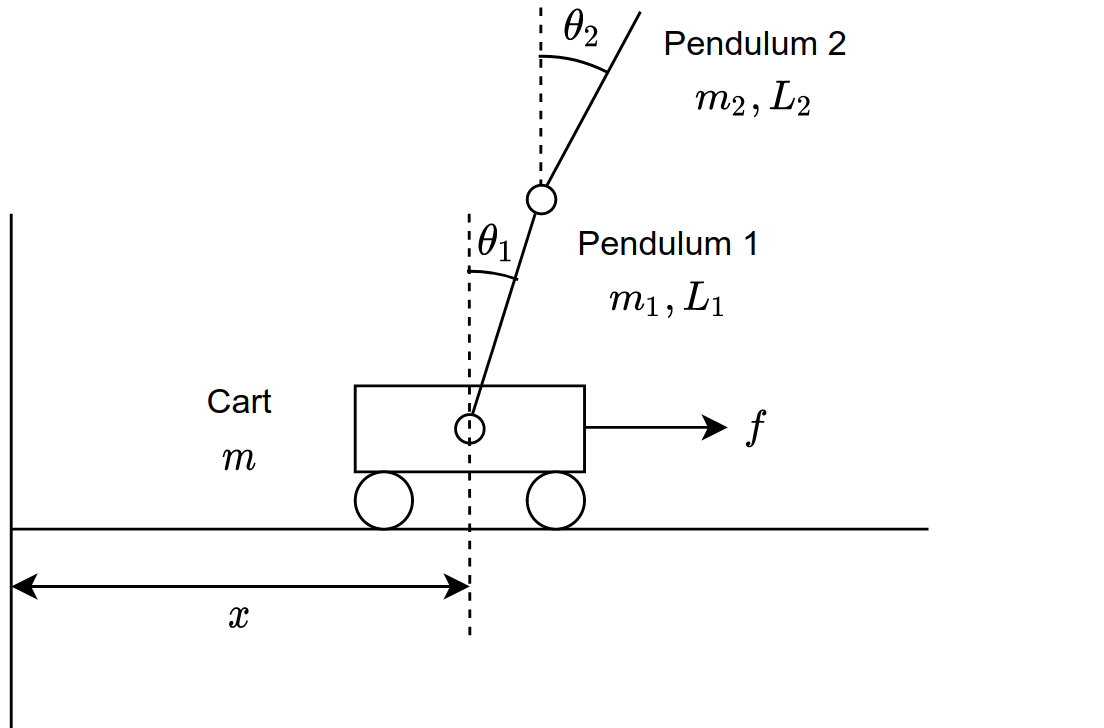
\includegraphics[width=2.5in]{fig01_cart001.png}
    \caption{Physical System}
    \label{fig_sim}
\end{figure}


\subsection{State Definition}
Suppose we have a continuous-time, nonlinear system presented in state space
form.
% ss form

\begin{equation}
    % \label{eq:6}
    \dot{x} = f(x,u),
\end{equation}
\begin{equation}
% \label{eq:7}
    y = h(x).
\end{equation}

whats f - prediction model
whats h - obs model
omit obs noise, it requires EKF??

Our goal is to stabilize the described highly nonlinear system in the upright
configuration

\subsection{Noise and Friction}
% paper

\subsection{Global Coordinate Frame}
We need to form a homogenous configuration space to present state variables
\(q, \theta_1, \theta_2\) by forming a global coordinate frame with \(x(t=0)\)
as the origin.
\begin{equation}
    \begin{split}
    % \label{eq:6}
    q_c = \begin{bmatrix}
    q \\
    0 \\
    \end{bmatrix}, ~~
    q_1 = \begin{bmatrix}
    q + l_1 \sin \theta_1 \\
    l_1 \cos \theta_1 \\
    \end{bmatrix}, \\
    % \label{eq:6}
    q_2 = \begin{bmatrix}
    q + l_1 \sin \theta_1 + l_2 \sin \theta_2 \\
    l_1 \cos \theta_1 + l_2 \cos \theta_2 \\
\end{bmatrix},
\end{split}
\end{equation}
\noindent
We denote position of point-masses for \(m_c\), \(m_1\), and
\(m_2\) by \(q_c, q_1, q_2 \in R^2\) on the x-y plane.
We seek to define our system in terms of these state variables. Thus, we define
state variable vector \(q(t)\) as
\begin{equation}
q = [q_c, q_1, q_2]^{T}
\end{equation}
In a later section, we formally rewrite state variable definitions independent of
time \(t\) via a linearization process. For simpler representation, we
denote state variable vector as \(q:=q(t)\).

\subsection{Other Considerations}
Noise and Friction modeling, process noise versus observation noise.

\section{Model Derivation}
% steps



\subsection{Equations of Motion}
As it is laid out in \emph{Lagrangian mechanics}; first we must obtain the Lagrangian
of the physical model, \(\mathcal{L}= K -P\). \(K\) and \(P\) represent the
\emph{kinetic} and \emph{potential} energies of the system. \(K\) is the total
kinetic energy from all three masses and in later sections, we will discuss
transforming \emph{Lagrangian mechanics} to \emph{Hamiltonian mechanics} by
replacing velocities with \emph{momenta}. Here, we define K as
\begin{equation}
    K = \frac{1}{2} m v^2 =~ \frac{1}{2} {m_c\|\dot{q_c}\|^2 + m_1\|\dot{q_1}\|^2 + m_2\|\dot{q_2}\|^2}.
\end{equation}

P denotes the overall potential energy of the system; but since the cart rolls
flat along the x-axis, it is inherently incapable of storing energy so we discard
it. P is obtained by
\begin{equation}
    P = g \left[ m_1 l_1 \cos \theta_1 + m_2 (l_1 \cos \theta_1 + l_2 cos \theta_2) \right]
\end{equation}
Where \(g \in R\) denotes gravitational acceleration.
Next, we envoke the \emph{Euler-Lagrange} equation to write the following ODE system
whose solution is the position and velocity configuration vector of the cart
and masses on the x-y plane, given the final time, previous state, system
dynamics, control input and disturbances.
\begin{equation}
    y(t) = f(t,q,\dot{q},u,\omega)
\end{equation}
\emph{The Lagrange Equations of Motions} are defined as
\begin{equation}
    Q = \frac{\partial\mathcal{L}}{\partial f_{i}} - \frac{d}{dt} \left( \frac{\partial \mathcal{L}}{\partial f_{i}}\right).
\end{equation}
Where \(Q\) represents the vector of sum of external forces acting on the plan.
\begin{equation}
    \mathcal{L} = \mathcal{L}(t, q, \dot{q})
\end{equation}
\begin{equation}
\begin{cases}
\begin{array}{rcl}
    u + \omega_1 -d_1 \dot{q} &=& \frac{d}{dt} \{\frac{\partial\mathcal{L}}{\partial\dot{q}}\}-\{\frac{\partial\mathcal{L}}{\partial q}\}\\
    \omega_2 -d_2 \dot{\theta_1} &=& \frac{d}{dt} \{\frac{\partial\mathcal{L}}{\partial\dot{\theta_1}}\}-\{\frac{\partial\mathcal{L}}{\partial \theta_1}\}\\
    \omega_3 -d_3 \dot{\theta_2} &=& \frac{d}{dt} \{\frac{\partial\mathcal{L}}{\partial\dot{\theta_2}}\}-\{\frac{\partial\mathcal{L}}{\partial \theta_2}\}\\
    \end{array}
\end{cases}
\end{equation}

So far our derivation has made our expressions more complicated but these steps are
necessary for capturing the full dynamical characteristics of the system. In the
following section, we derive the continuous-time nonlinear model of the described
system. Moreover in \emph{Optimal Control} section, we briefly explain how one
could derive \emph{the general optimal control solution} for a \emph{positive
definite and semidefinite energy system} with known characteristics.
Moreover, we intuitively explain and reference why we could consider the solution
space to such an ODE as \emph{smooth manifold} that maps current and future state
through recursion and its energy state decays towards a local minima.


\subsection{Continues-Time, Nonlinear Model}
We used MATLAB Symbolic Math Toolbox to derive the resultant ODE. Obtaining
symbolic or implicit expressions of our ODE will allow us to analytically derive
to the optimal solution.
\begin{equation}
\text{\scriptsize $
% \begin{cases}
\begin{array}{rcl}
    u + \omega_1 -d_1 \dot{q} &=& (m_c+m_1+m_2)\ddot{q}+l_1(m_1+m_2)\ddot{\theta_1} \cos \theta_1\\
    & & + m_2 l_2 \ddot{\theta_2} \cos \theta_2 - l_1 (m_1+m_2) \dot{\theta_1}^2 \sin \theta_1 \\
    & & - m_2 l_2 \dot{\theta_2}^2 \sin \theta_2\\
    \omega_2 -d_2 \dot{\theta_1} &=& l_1 (m_1+m_2) \ddot(q) \cos \theta_1
    +l_1^2 (m_1+m_2) \ddot{\theta_1}\\
    & & +l_1 l_2 m_2 \ddot{\theta_2} \cos (\theta_1 - \theta_2)+ l_1 l_2 m_2 \dot{\theta_2}^2 \sin(\theta_1 - \theta_2) \\
    & & - g(m_1+m_2) l_1 \sin \theta_1 \\
    \omega_3 -d_3 \dot{\theta_2} &=& l_2 m_2 \ddot{q} \cos \theta_2
    + l_1 l_2 m_2 \ddot{\theta_1} \cos (\theta_1 -\theta_2)
    + l_2^2 m_2 \ddot{\theta_2}\\
    & & -l_1 l_2 m_2 \dot{\theta_1}^2 \sin (\theta_1 - \theta_2)
    - l_2 m_2 g \sin \theta_2\\
    \end{array}
% \end{cases}
$}
\end{equation}

\subsection{Optimal Control}
% define
% in other words
% so we do this

\subsection{Linearization}
First, we rewrite the equations of motion into matrix form to batch acceleration,
velocity, and position terms into separate matrices. A second order representation
of the physical system is sufficient to provide an accurate enough estimate,
per \emph{Taylor Series Linearization} method. This is an important step as
identifying system dynamics lies at the heart of \emph{Optimal Control}.
\begin{equation}
D(q) \ddot{q} + C(q, \dot{q}) \dot{q} + G(q) = Hu
\end{equation}
where matrix functions \(D(q) \ddot{q} + C(q, \dot{q}) \dot{q} + G(q)\)
represent systems dynamics with respect to time,
current state and previous state. Time variable \(t\) is omitted to simplify
notation. The system energy state (left hand side of
above EOM) is presented in relation to external forces \(Hu\) acting on the
system. Vector \(u \in R^1\) represents external input forces vector and matrix
\(H\) represents its relationship with state variable functions. Matrix
functions \(D(q),~C(q, \dot{q}),~G(q)\) and vector H are define as

\begin{equation}
% \text{\scriptsize $
% \begin{cases}
% \begin{array}{rcl}
    D(q) = \begin{pmatrix}

    \end{pmatrix}
% \end{array}
% \end{cases}
% $}
\end{equation}


We need to rewrite the EOM in the following
matrix form to obtain the final ODE. Per \emph{Lyapunov
Control Function theory} (LCF) for autonomous dynamical systems and
\emph{LaSalle's}, we can assume there exists a
\emph{Optimal Control Trajectory} or \emph{Hamiltonian Flow} for a valid
initial condition if the LCF is \emph{positive definite} or \emph{positive
semi-definite}.


Moreover, the energy function describing the system must be \emph{symmetric} and \emph{positive definite} in order to form \emph{stable} control trajectory.

\begin{equation}
M(q)\dot{q} = A(q)q + Bu
\end{equation}

Where \emph{positive definite} or \emph{positive semi-definite} constraints are
evaluated by computing the determinant of \(M\).
\begin{equation}
det(M) > 0;~ \forall q
\end{equation}
Such that, the final ODE can be written as
\begin{equation}
    \dot{q} = M(q)^{-1}(A(q)q + Bu)
\end{equation}
To make remove the time index and make the ODE fully \emph{isomorphic}, we
define a new variable state vector as
\begin{equation}
    x:=
    \begin{bmatrix}
        y \\
        \dot{y}\\
    \end{bmatrix}
\end{equation}

L(x, u) =
 x T
 Qx + uT Ru


we
\subsection{Discrete, Linear Model}
\begin{equation}
\begin{array}{rcl}
    x &=& Ax + Bu \\
    y &=& \dot{x} \\
\end{array}
\end{equation}

where A and B are defined as
\begin{equation}
    A =
\begin{bmatrix}
        0 & I \\
        D^{-1} \frac{\partial G}{\partial q} & 0 \\
\end{bmatrix}
\end{equation}

\begin{equation}
    B =
\begin{bmatrix}
    0 \\
    D^{-1} H\\
    \end{bmatrix}
    \end{equation}

\subsection{Linear Quadratic Regulator Solution}
So far, we have modeled, linearized, and discretized our system using state
space general form. In the process, we systematically reduced the solution space
complexity by replacing time \(t\) and velocity dimension as linear products of
current and previous states. This allows us to analytically derive a general
form optimal solution. But before we reach that step, we need to define a
general \emph{Cost Function} \(J\) that only depends on absolute minimal parameters,
which we will later optimize to arrive to a \emph{minimal surface}. Quadratic
performance index \(J \) is
defined as [see page 24 of Optimal control - now we can optimize similar to static cases]
\begin{equation}
J(x,u) = \frac{1}{2}x^{T}Q x + \frac{1}{2}u^{T}Ru
\end{equation}
whose solution is the minimal cost or minimum-energy input required for the
system to reach local minima, for any given initial state. Next, we minimize \(J\)
which will yield the state feedback weight vector \(K\) and is obtained by
recursively solving the dynamic \emph{Riccati} equation.
It is important to note that calculation of Quadratic losses are carried out by
performing dot product of state vector with its transpose and energy magnitude.


\section{Simulation and Animation}
For this project, both MATLAB and Python were used at different stages of the
development. Besides symbolic math derivation, MATLAB Control Toolbox was used
to check Python ODE simulation output and to obtain the LQR solution. MATLAB is
the gold-standard of scientific numerical analysis and Python is versaltile and
rich with high level feature. Various Python-based control system libraries were
explored and considered but were abandoned after observing variations in the
\emph{control vector} parameters. The LQR solution is expected to be optimal for
\emph{Lyapunov energy systems} and variations in the solution raises doubts
about numerical integrity of the computation process. For that reason, derivations
and control solutions used in this work are consistent with MATLAB.

Various Python libraries are used to simulate, animate and analyze model dynamics.
Pymunk and Pygame libraries are used create a 2D physics-based simulation
environment. Pyglet library (based on OpenGL) is used to create the animation,
figure \ref{fig_000_anim}. Source code for the animation and graphics are base
on examples and documentation provided by the authors \cite{pymunk}.


\begin{figure}[!t]
    \centering
    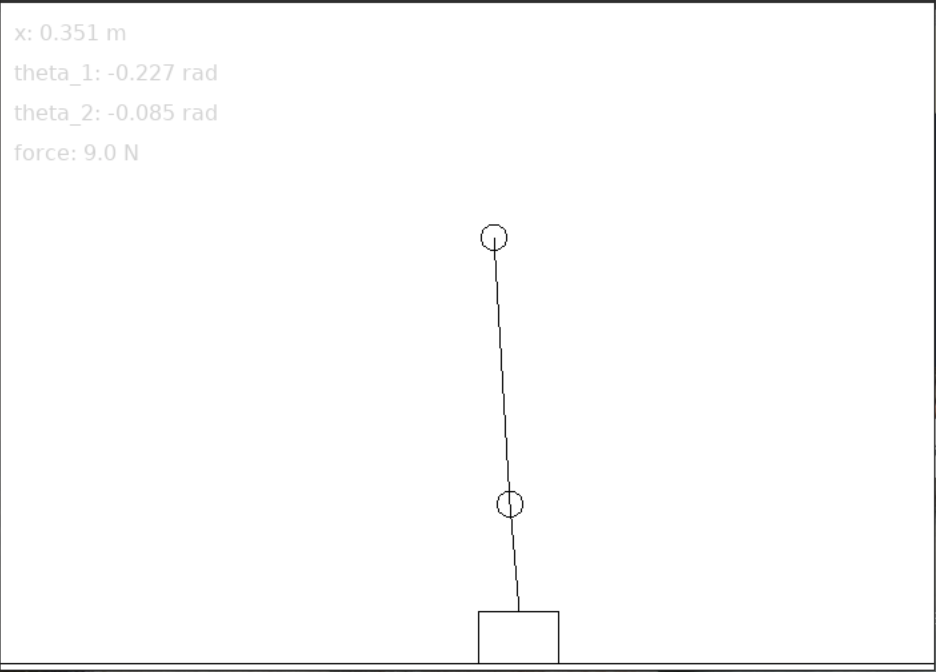
\includegraphics[width=2.5in]{fig_000_anim.png}
    \caption{Animation of Double Inverted Pendulum}
    \label{fig_000_anim}
\end{figure}


\subsection{Experiment I}
In the first experiment, we perform a set of tests with the goal of studying
system stability with respect to changes in model parameters.






% Note that IEEE typically puts floats only at the top, even when this
% results in a large percentage of a column being occupied by floats.


% An example of a double column floating figure using two subfigures.
% (The subfig.sty package must be loaded for this to work.)
% The subfigure \label commands are set within each subfloat command, the
% \label for the overall figure must come after \caption.
% \hfil must be used as a separator to get equal spacing.
% The subfigure.sty package works much the same way, except \subfigure is
% used instead of \subfloat.
%

% \begin{figure}[!t]
%     \centering
%     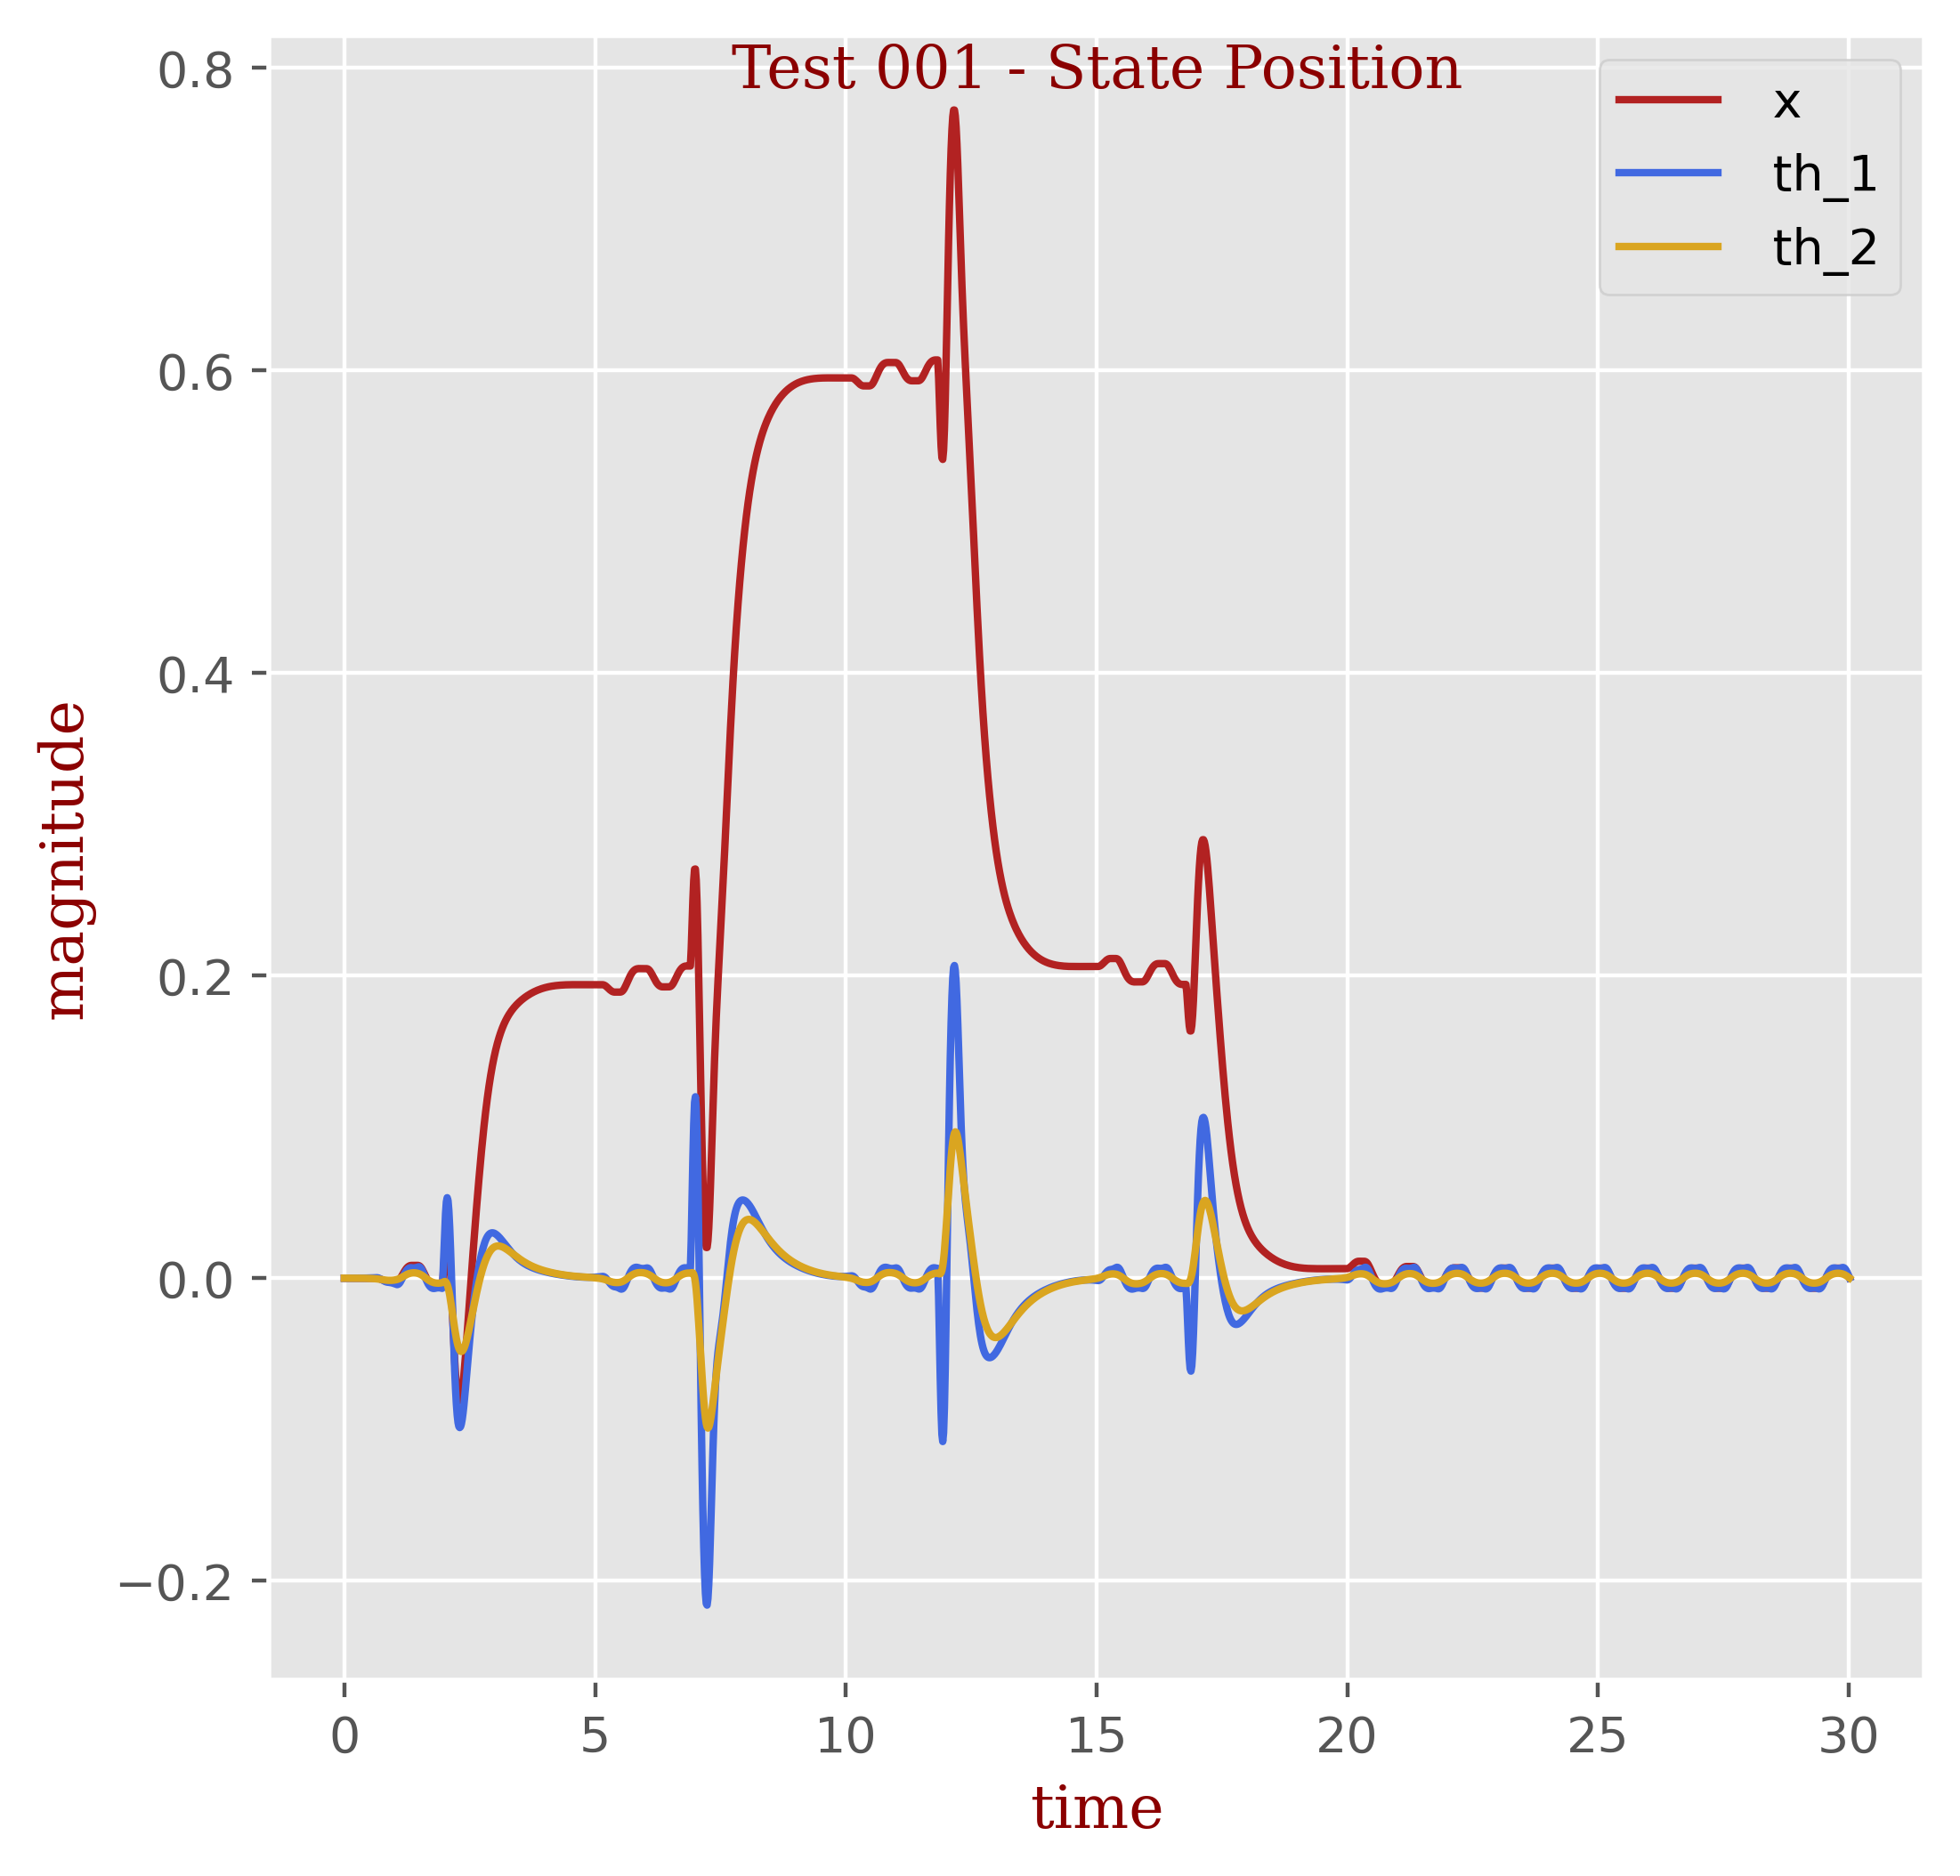
\includegraphics[width=2.5in]{Test 001_State_Position.png}
%     \centering
%     % \caption{Test 001 - Position}
%     \label{fig_T001_pos}
%     \centering
% \end{figure}

% \begin{figure}[!t]
%     \centering
%     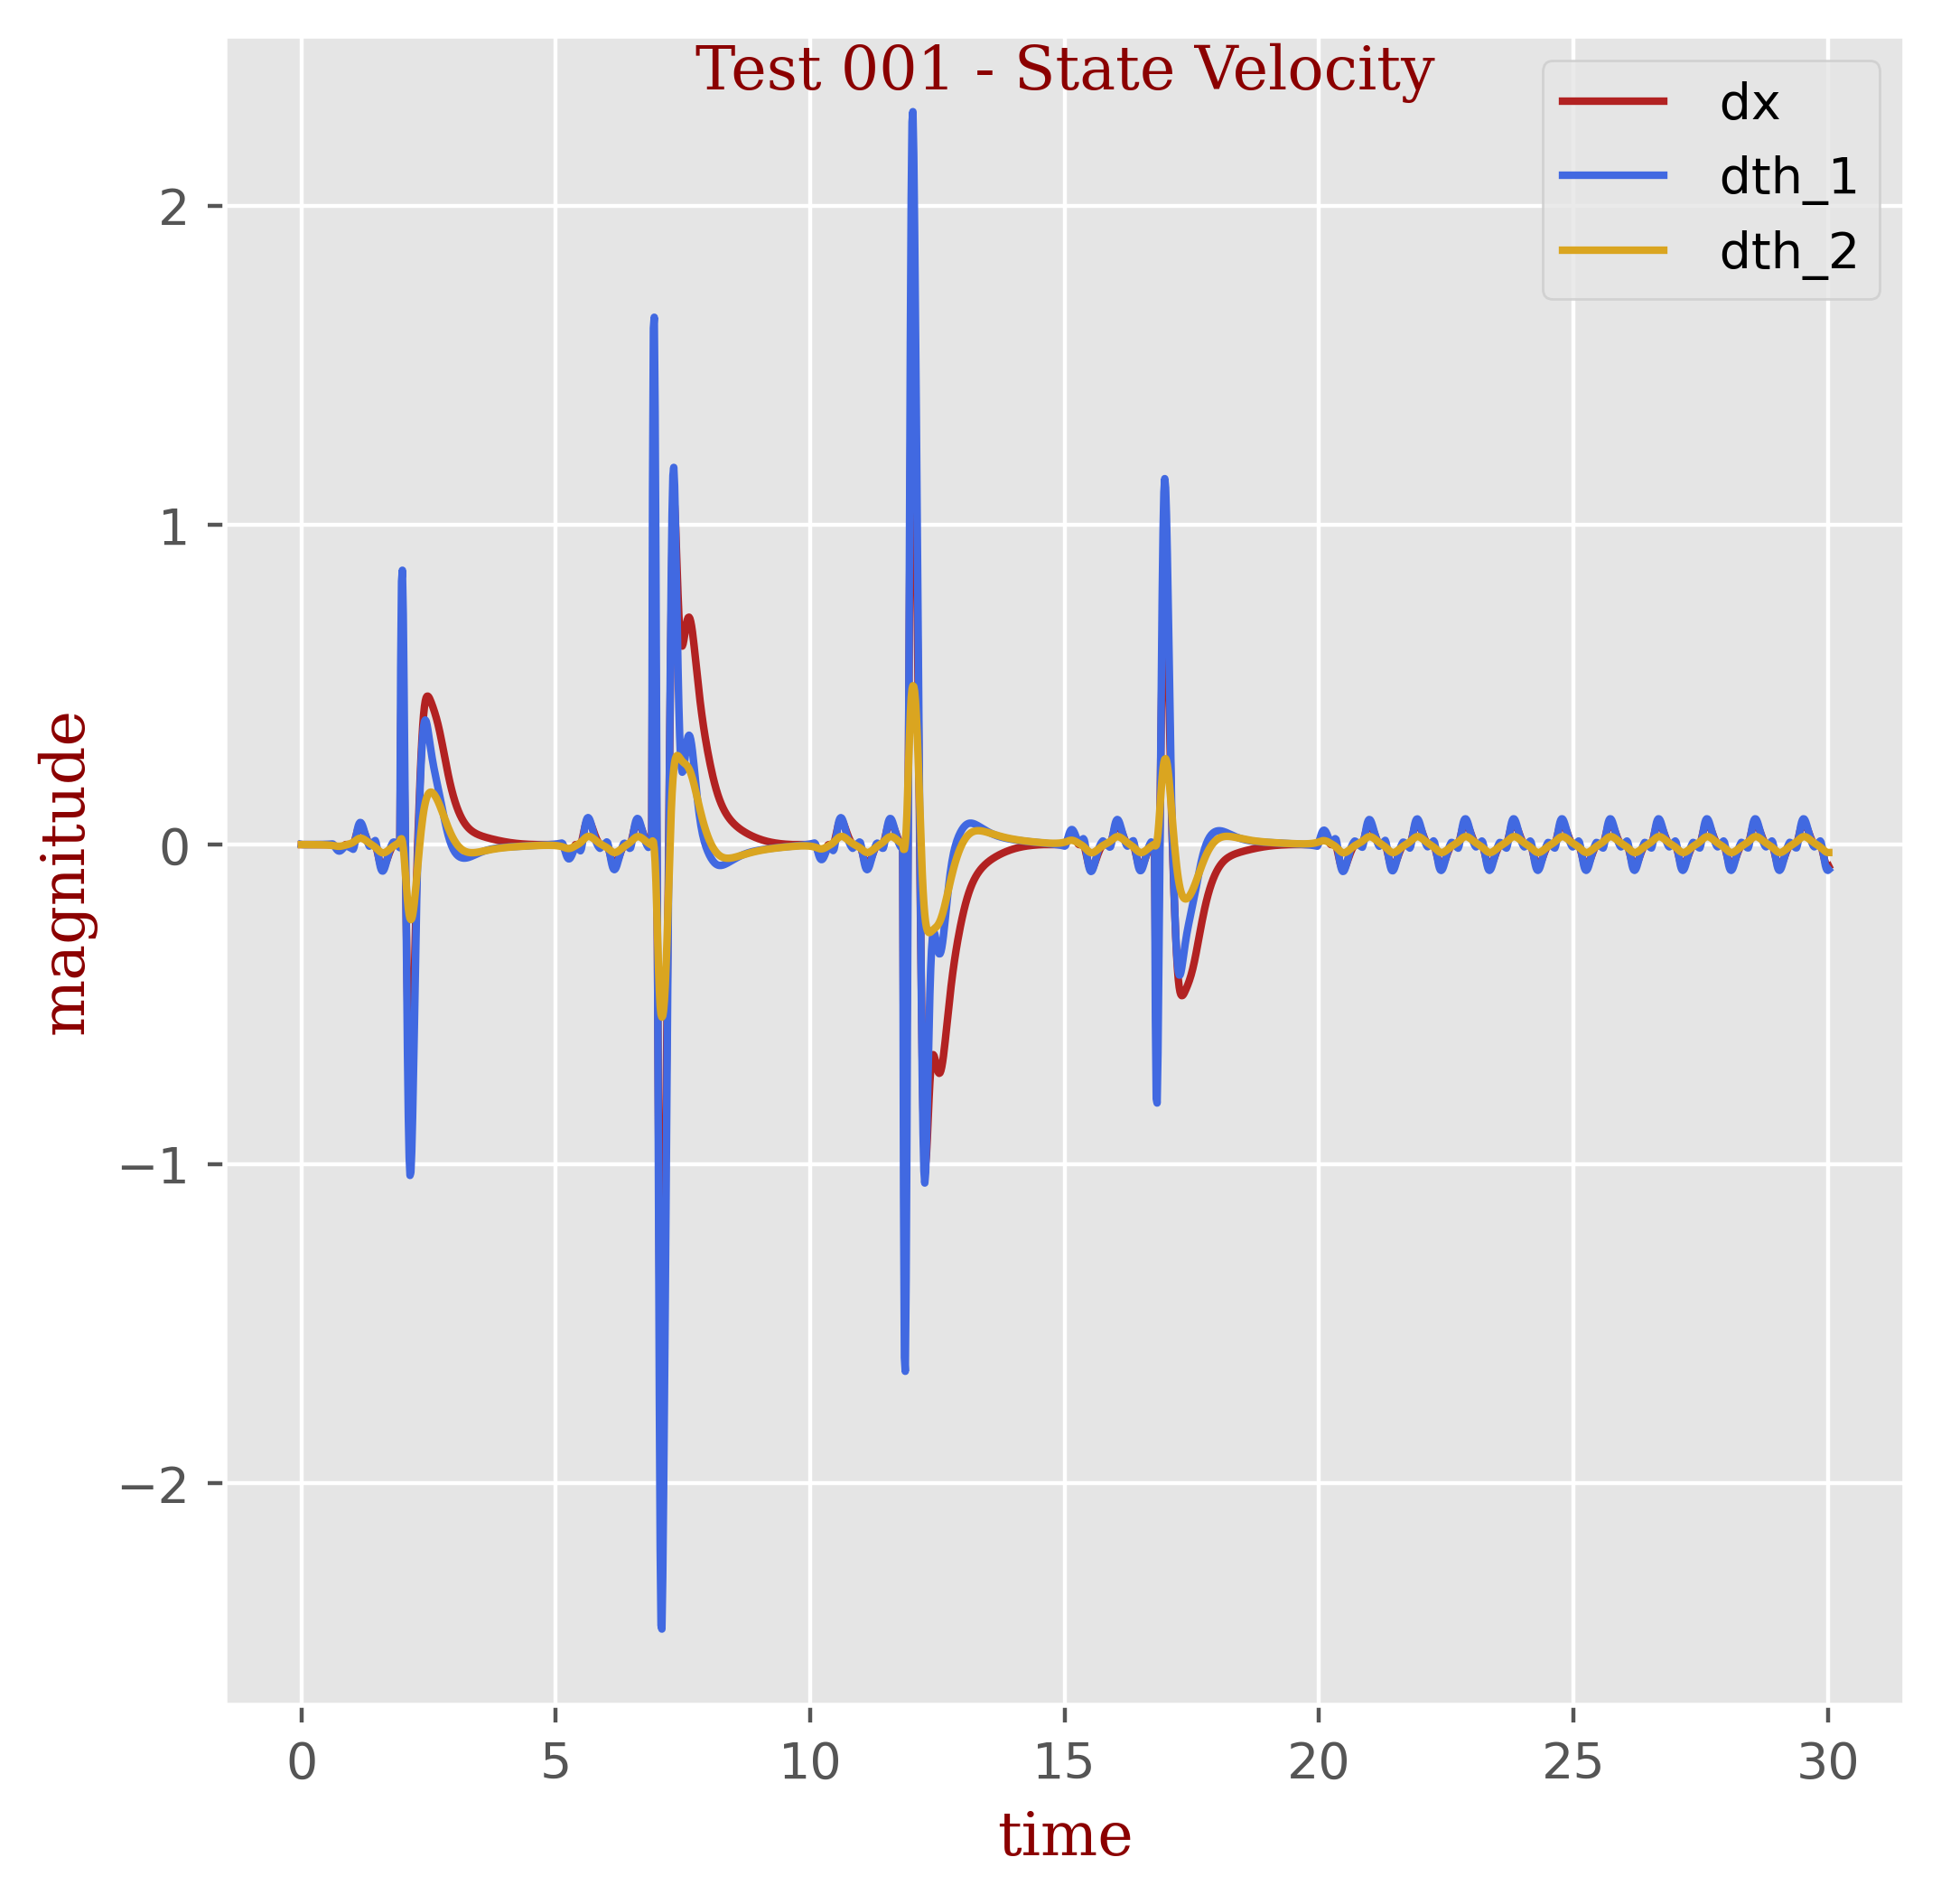
\includegraphics[width=2.5in]{Test 001_State_Velocity.png}
%     \centering
%     % \caption{Test 001 - Velocity}
%     \label{fig_T001_vel}
%     \centering
% \end{figure}

% \begin{figure}[!t]
%     \centering
%     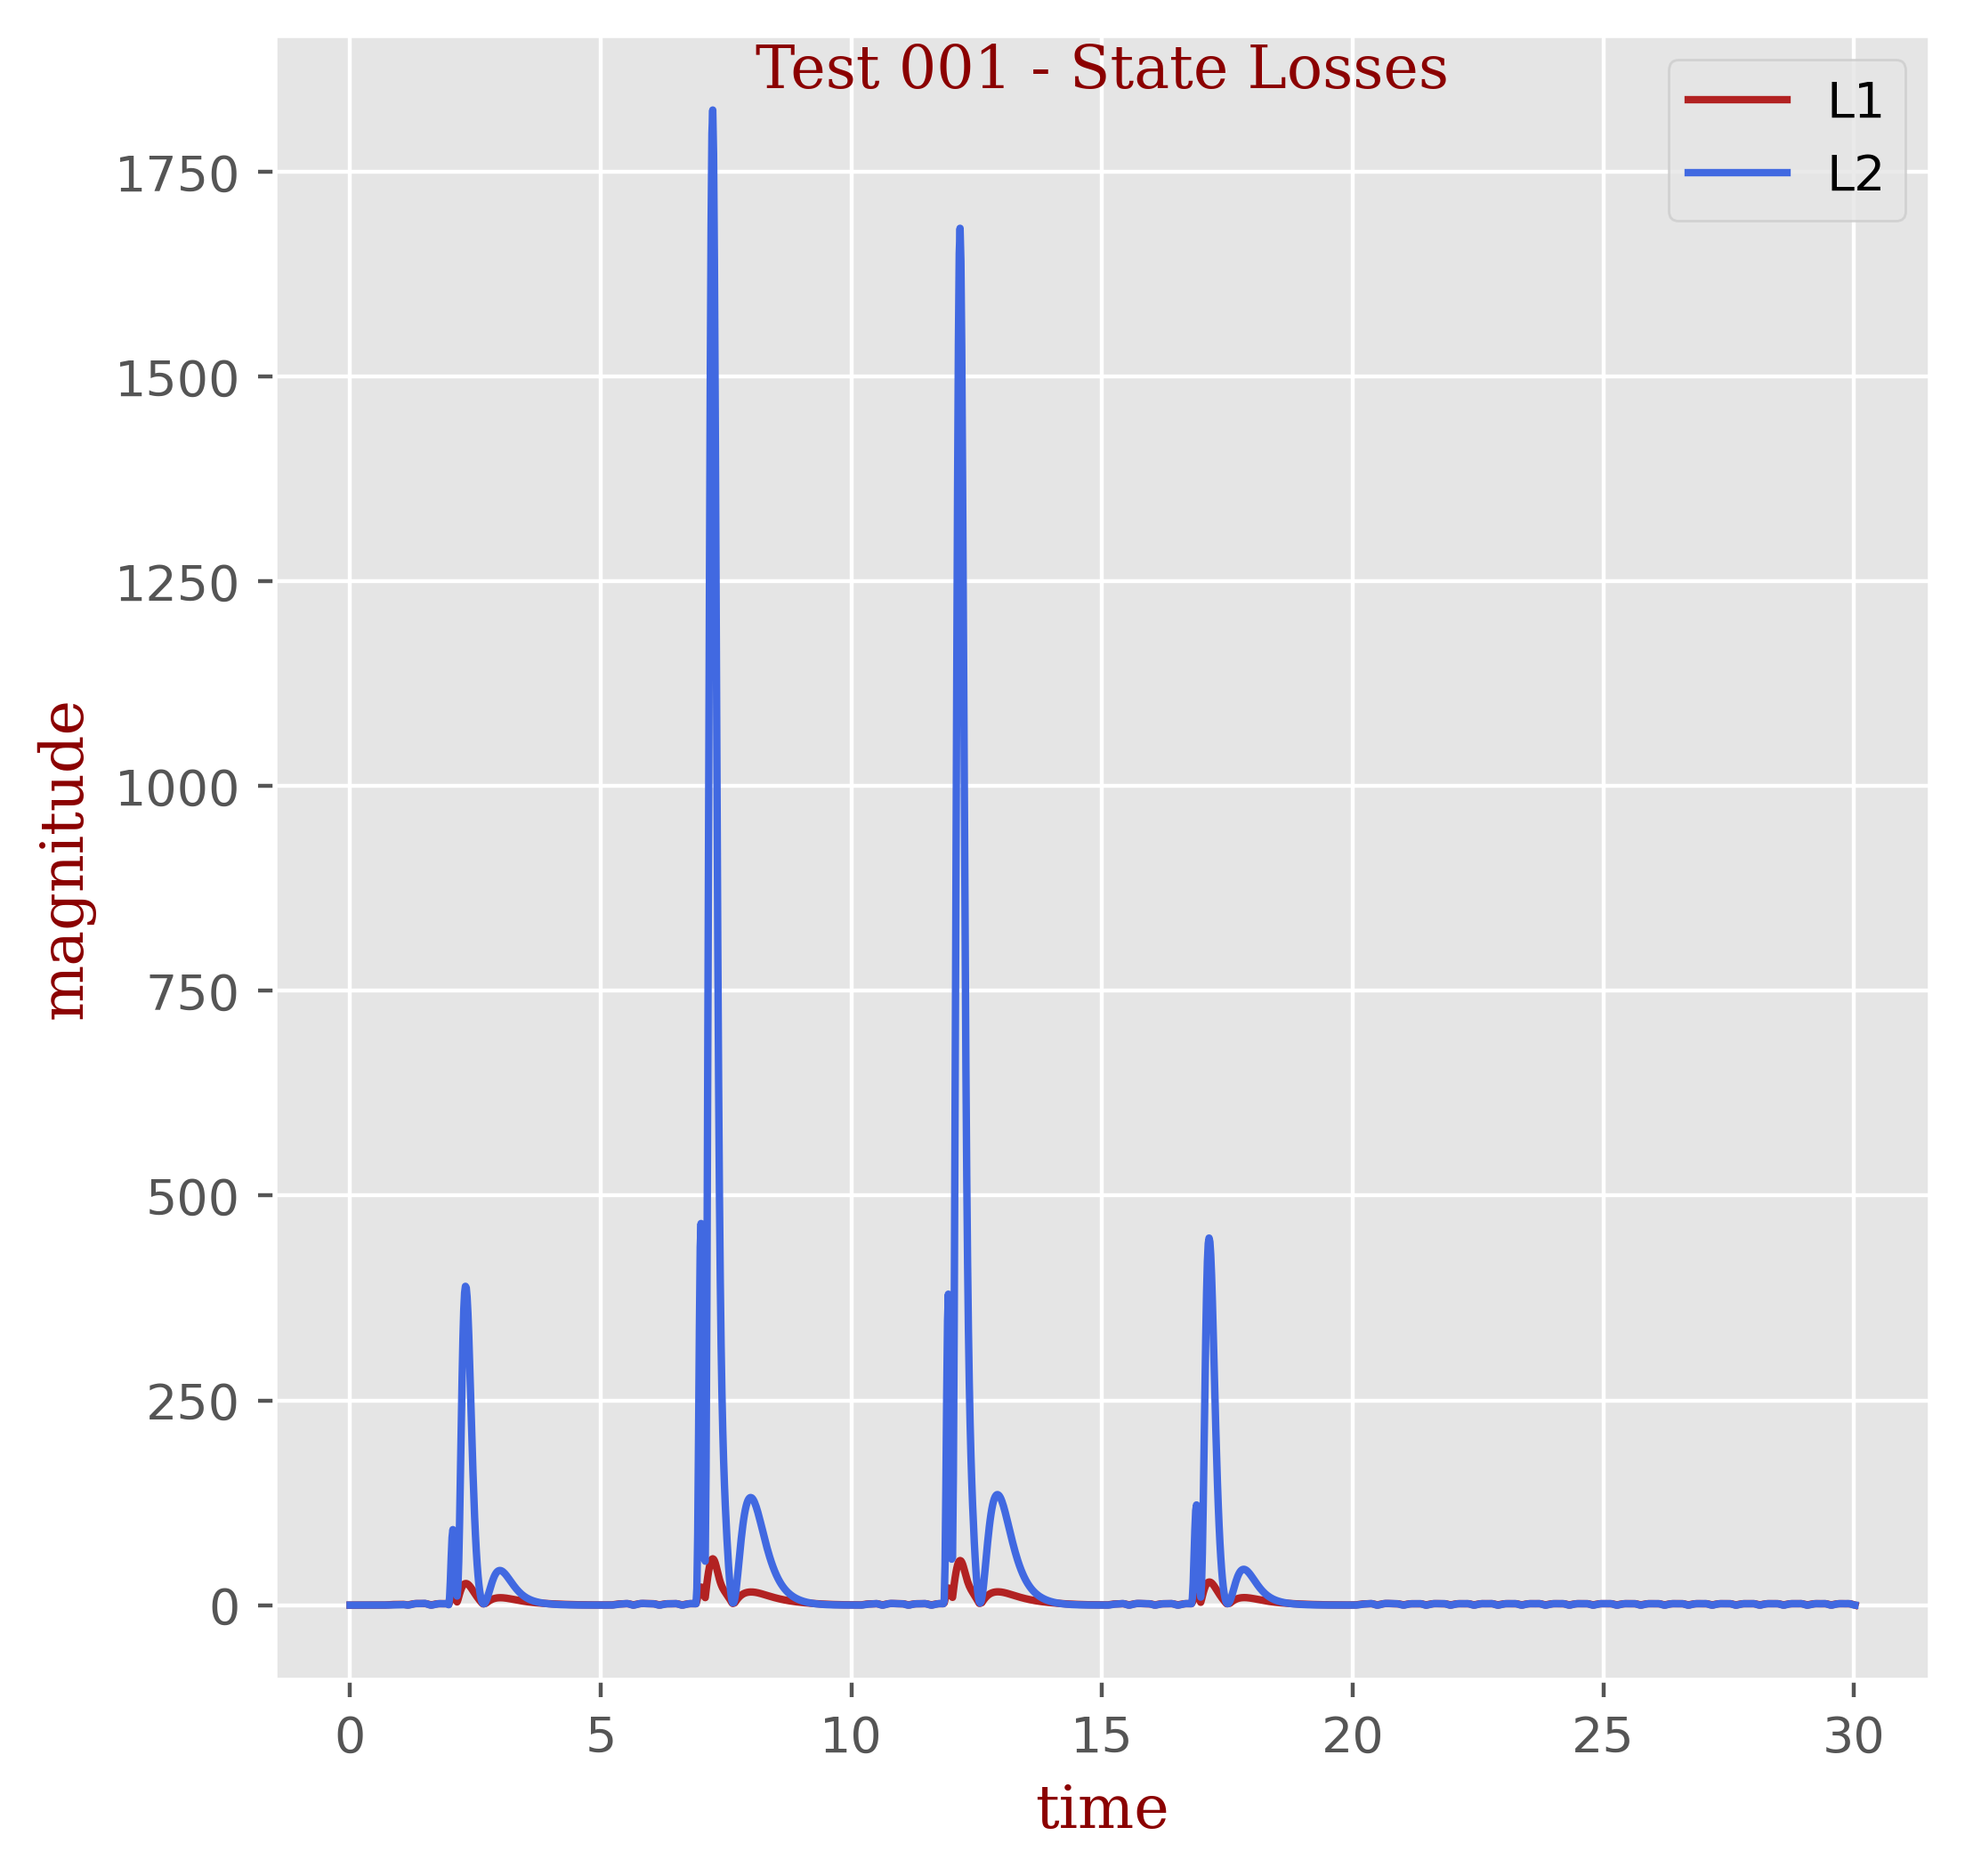
\includegraphics[width=2.5in]{Test 001_State_Losses.png}
%     \centering
%     % \caption{Test 001 - Losses}
%     \label{fig_T001_los}
%     \centering
% \end{figure}



% \begin{figure}
%     \begin{subfigure}[b]{0.05\textwidth}
%         \centering
%         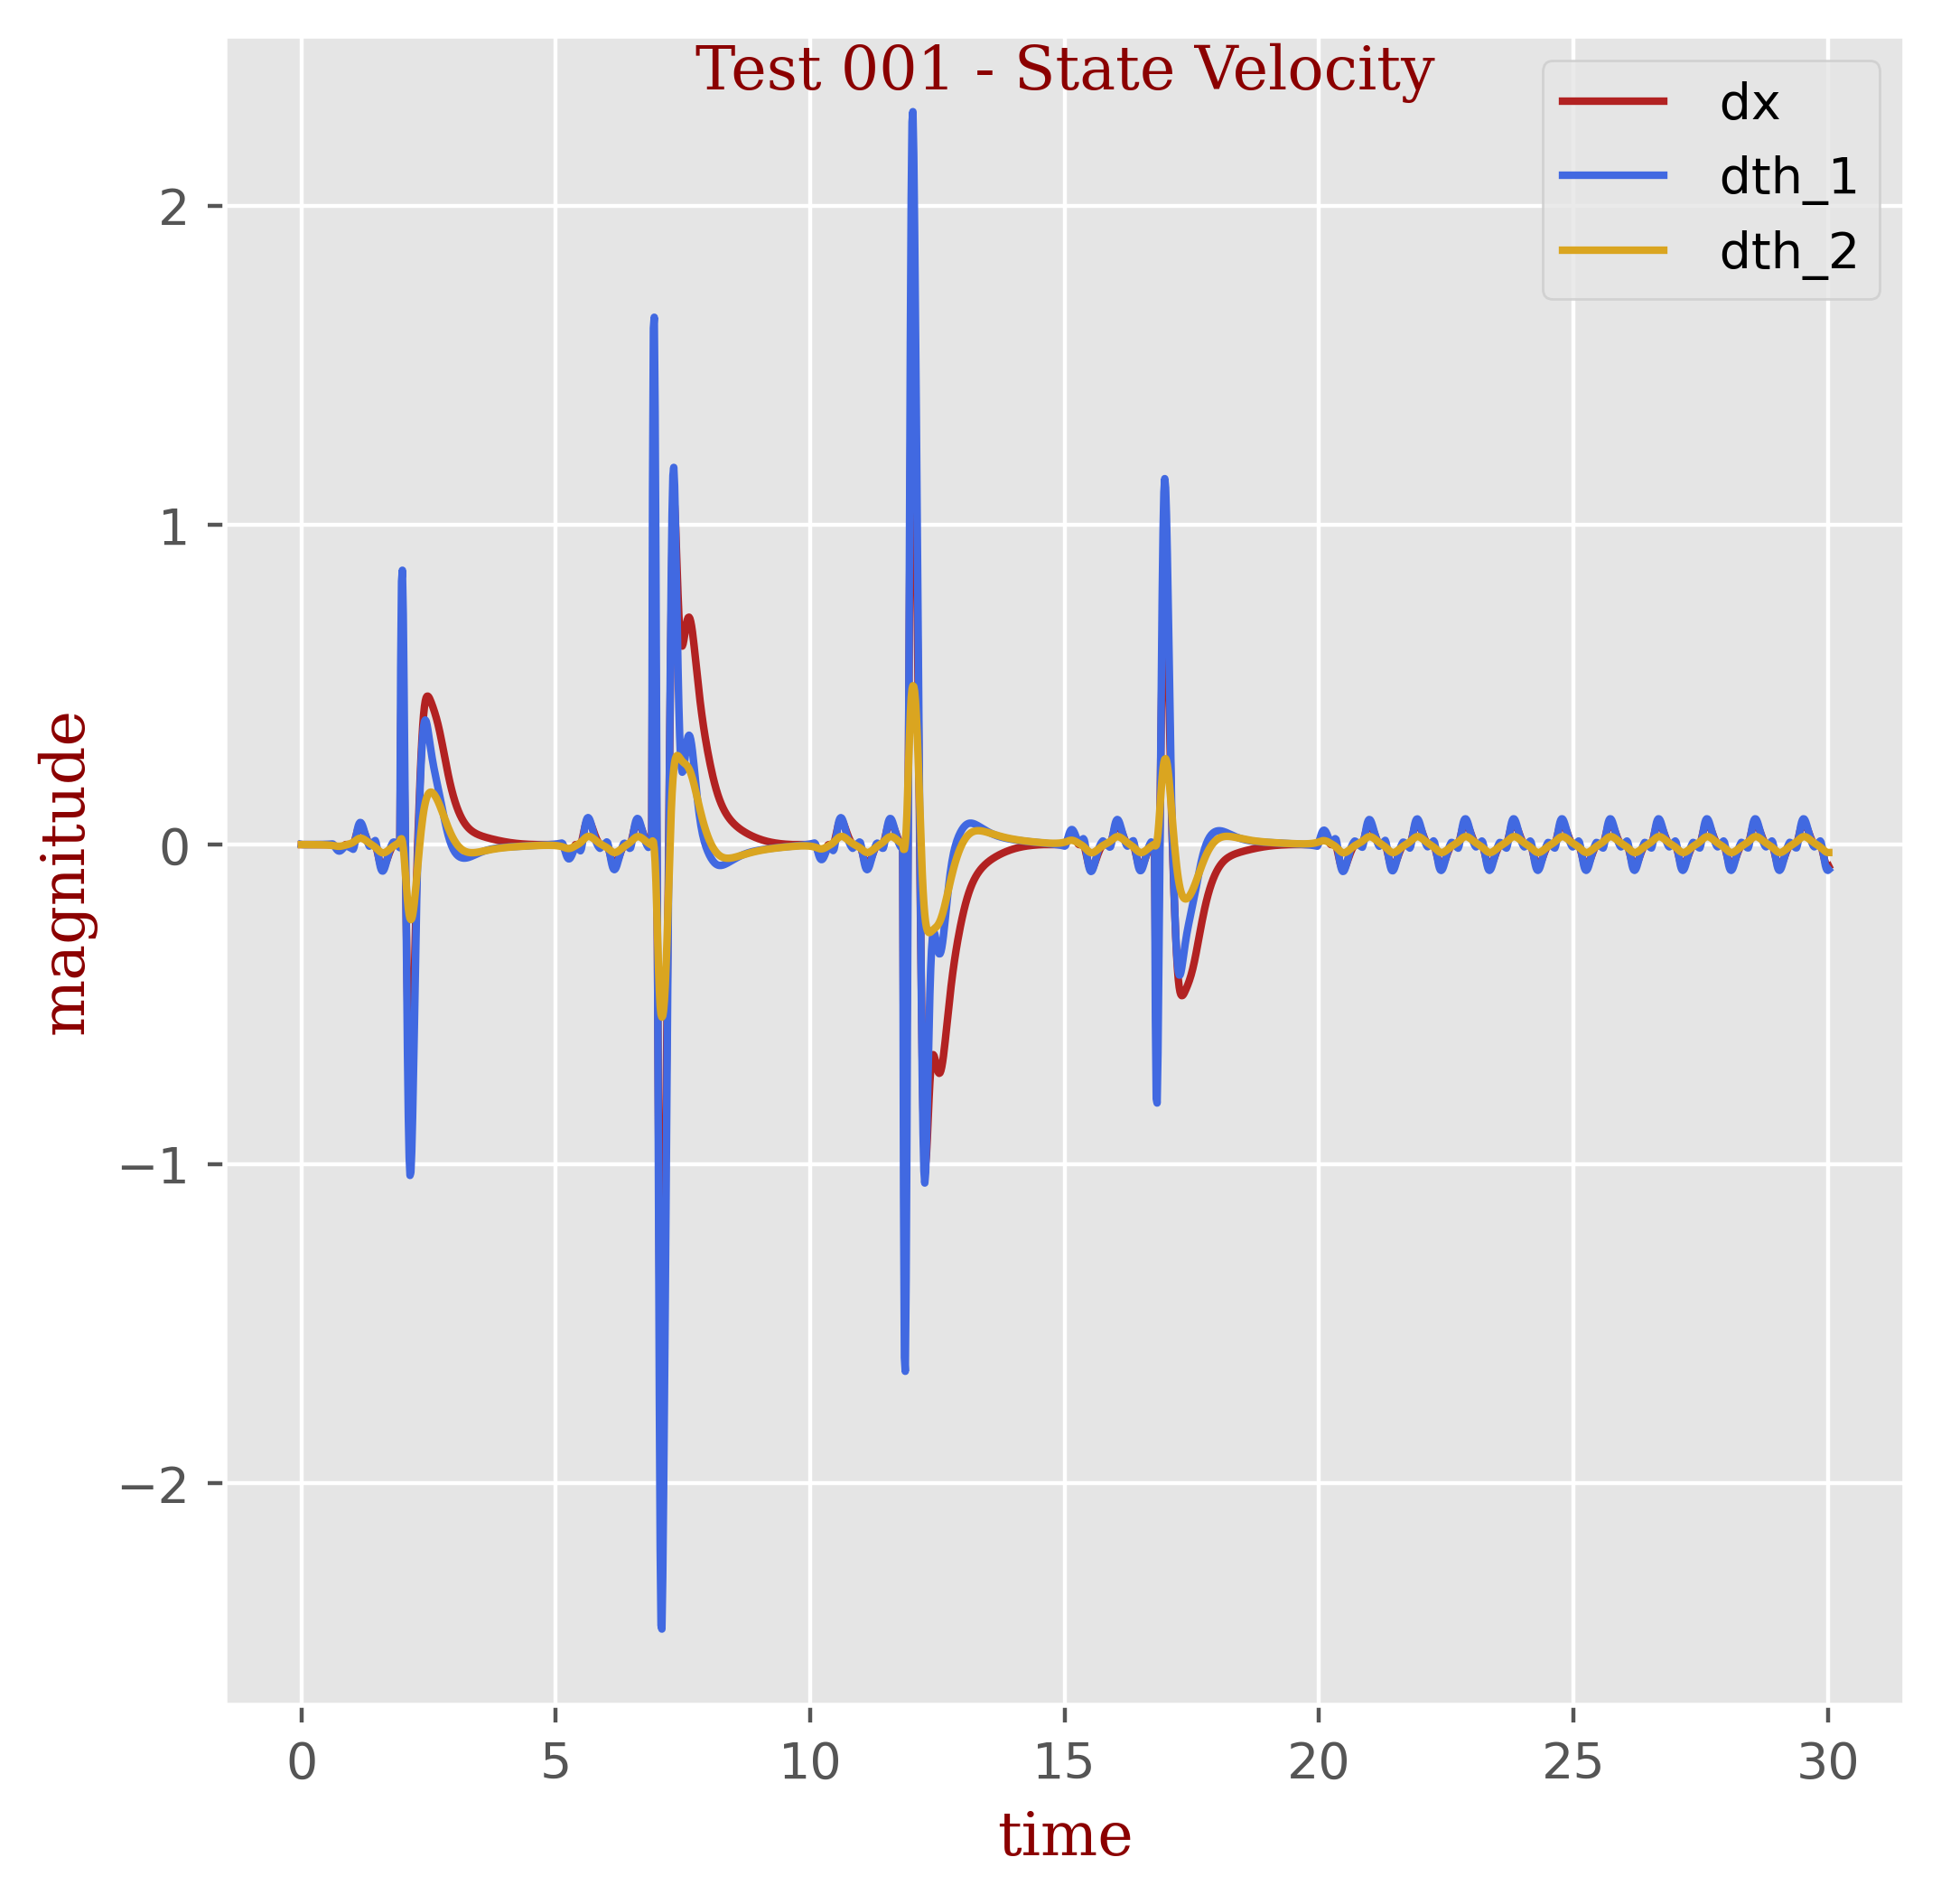
\includegraphics[width=\textwidth]{Test 001_State_Velocity.png}
%     % \caption{Test 001 - Position}
%     \label{fig_T001_pos}
%     \end{subfigure}
%     \hfill
%     \begin{subfigure}[b]{0.05\textwidth}
%         \centering
%         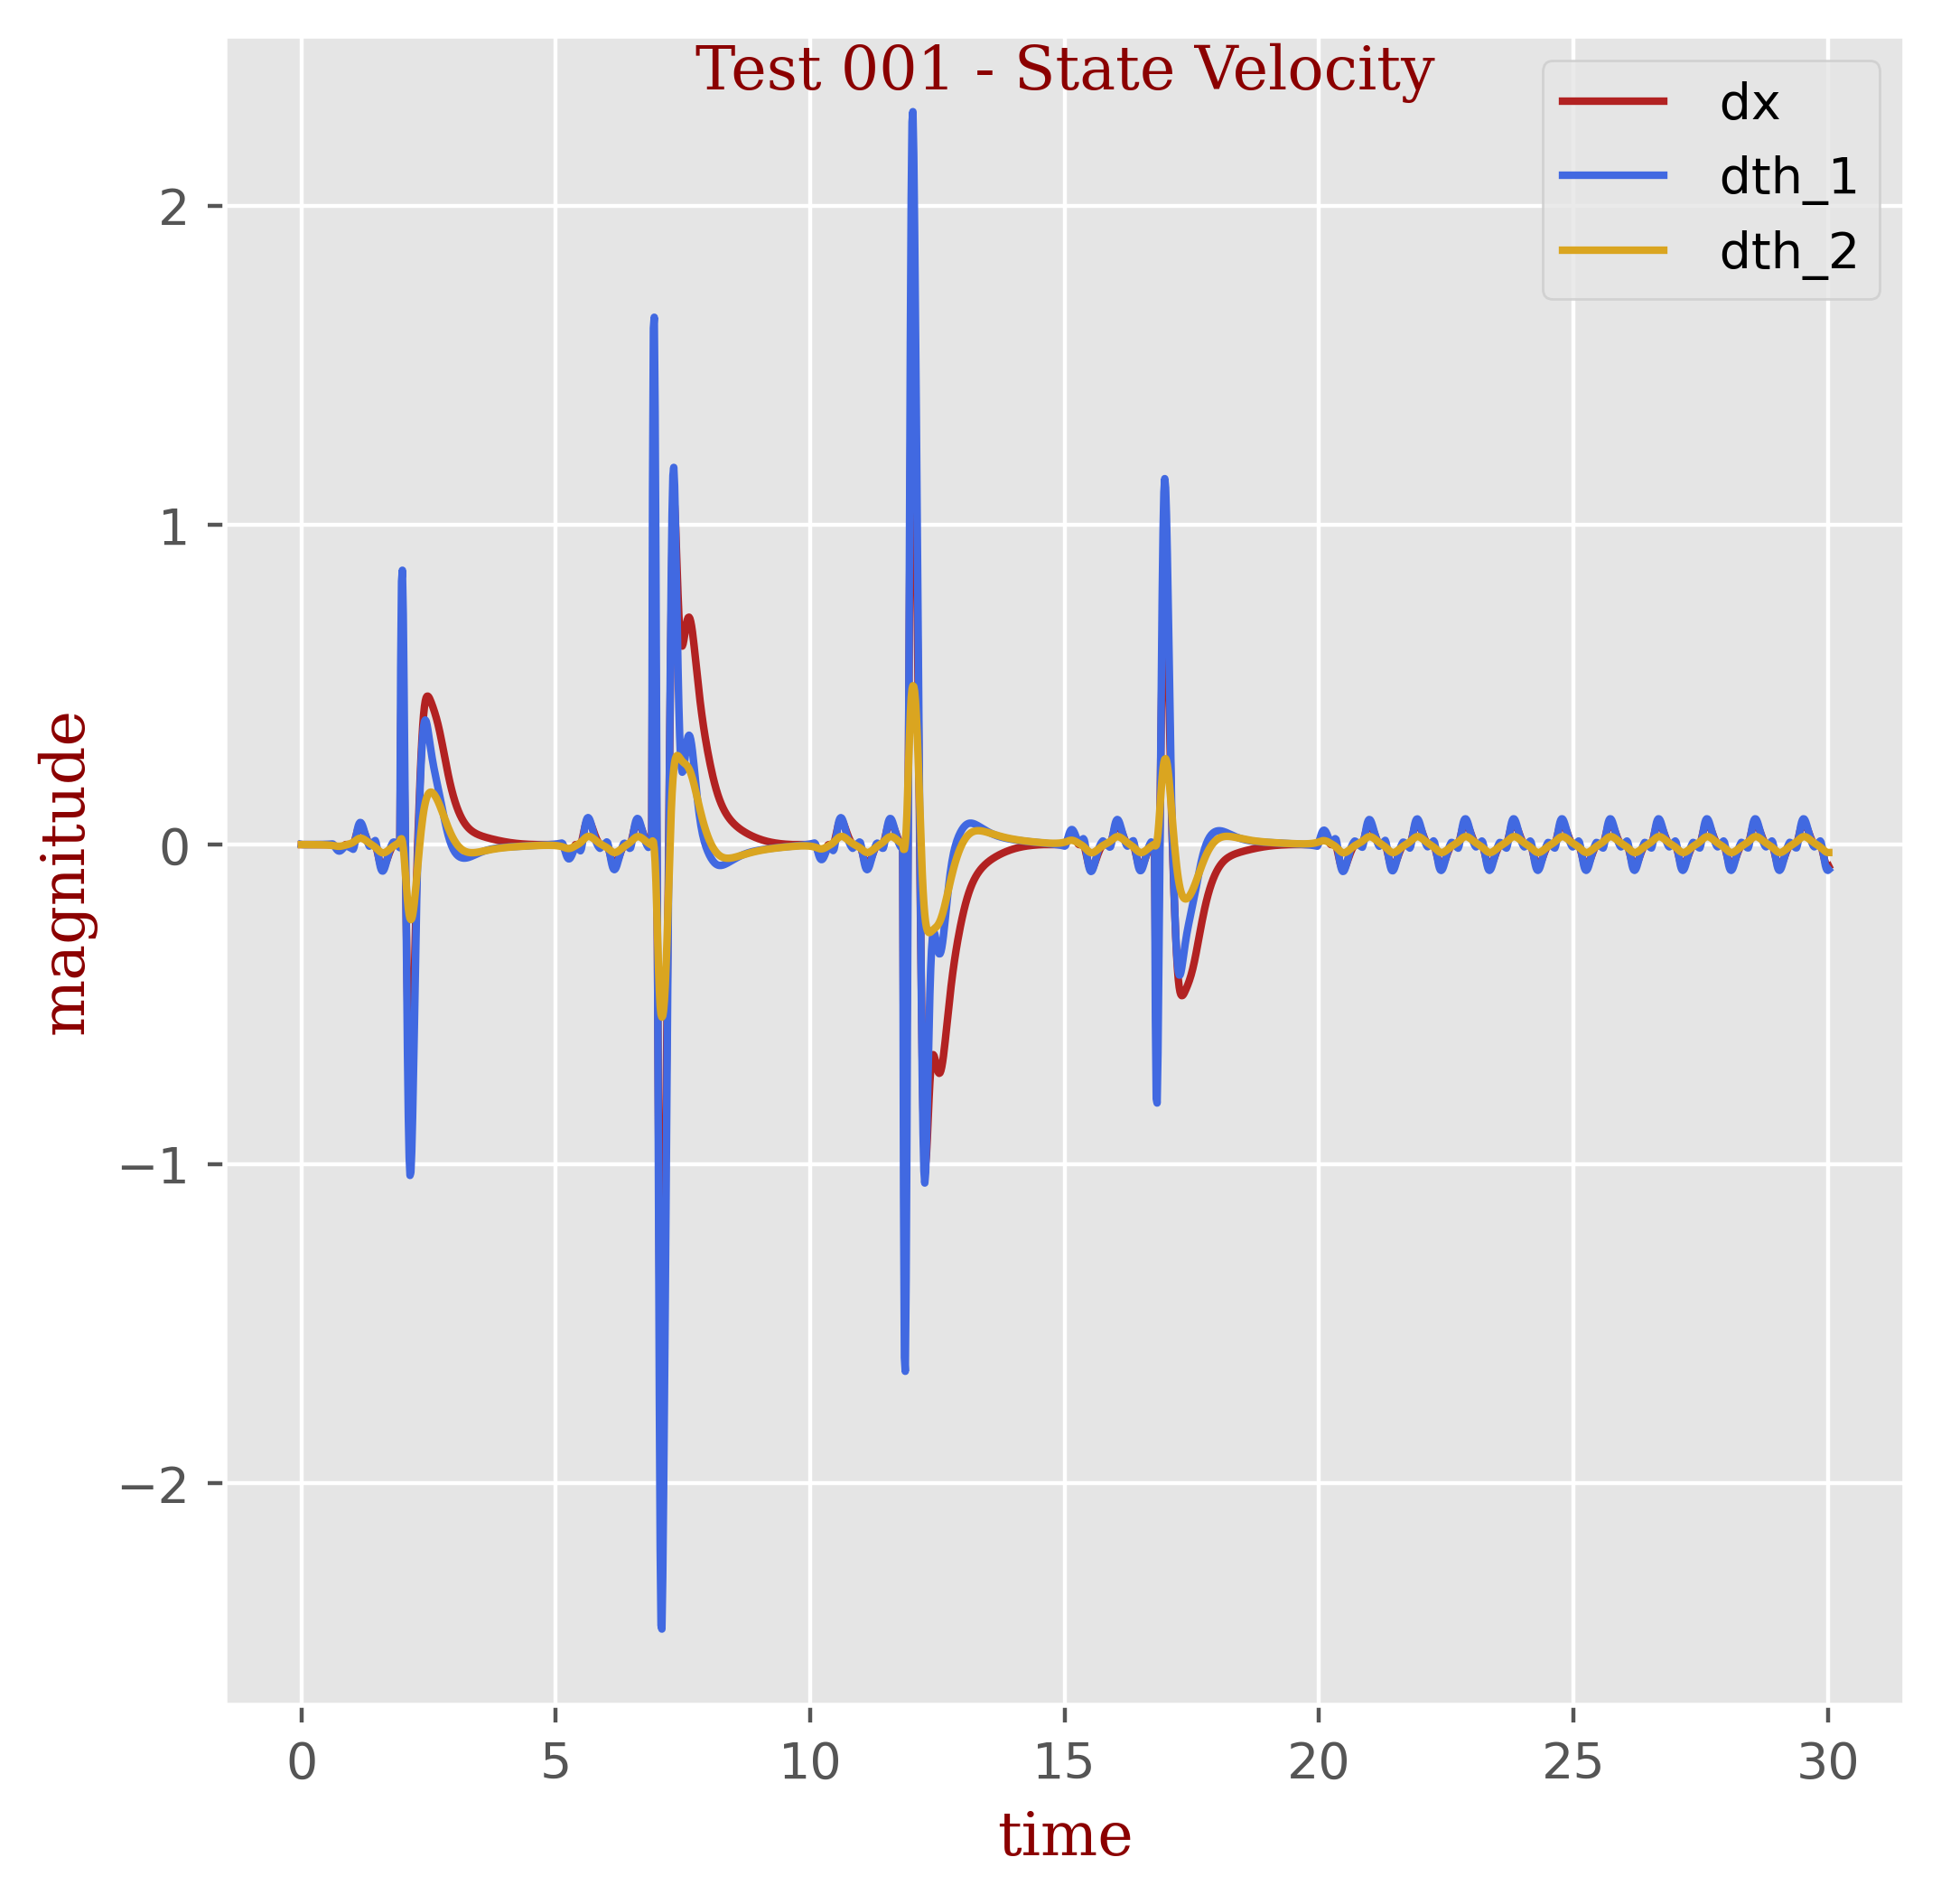
\includegraphics[width=\textwidth]{Test 001_State_Velocity.png}
%         \centering
%         % \caption{Test 001 - Velocity}
%         \label{fig_T001_vel}
%     \end{subfigure}
%     \hfill
%     \begin{subfigure}[b]{0.05\textwidth}
%         \centering
%         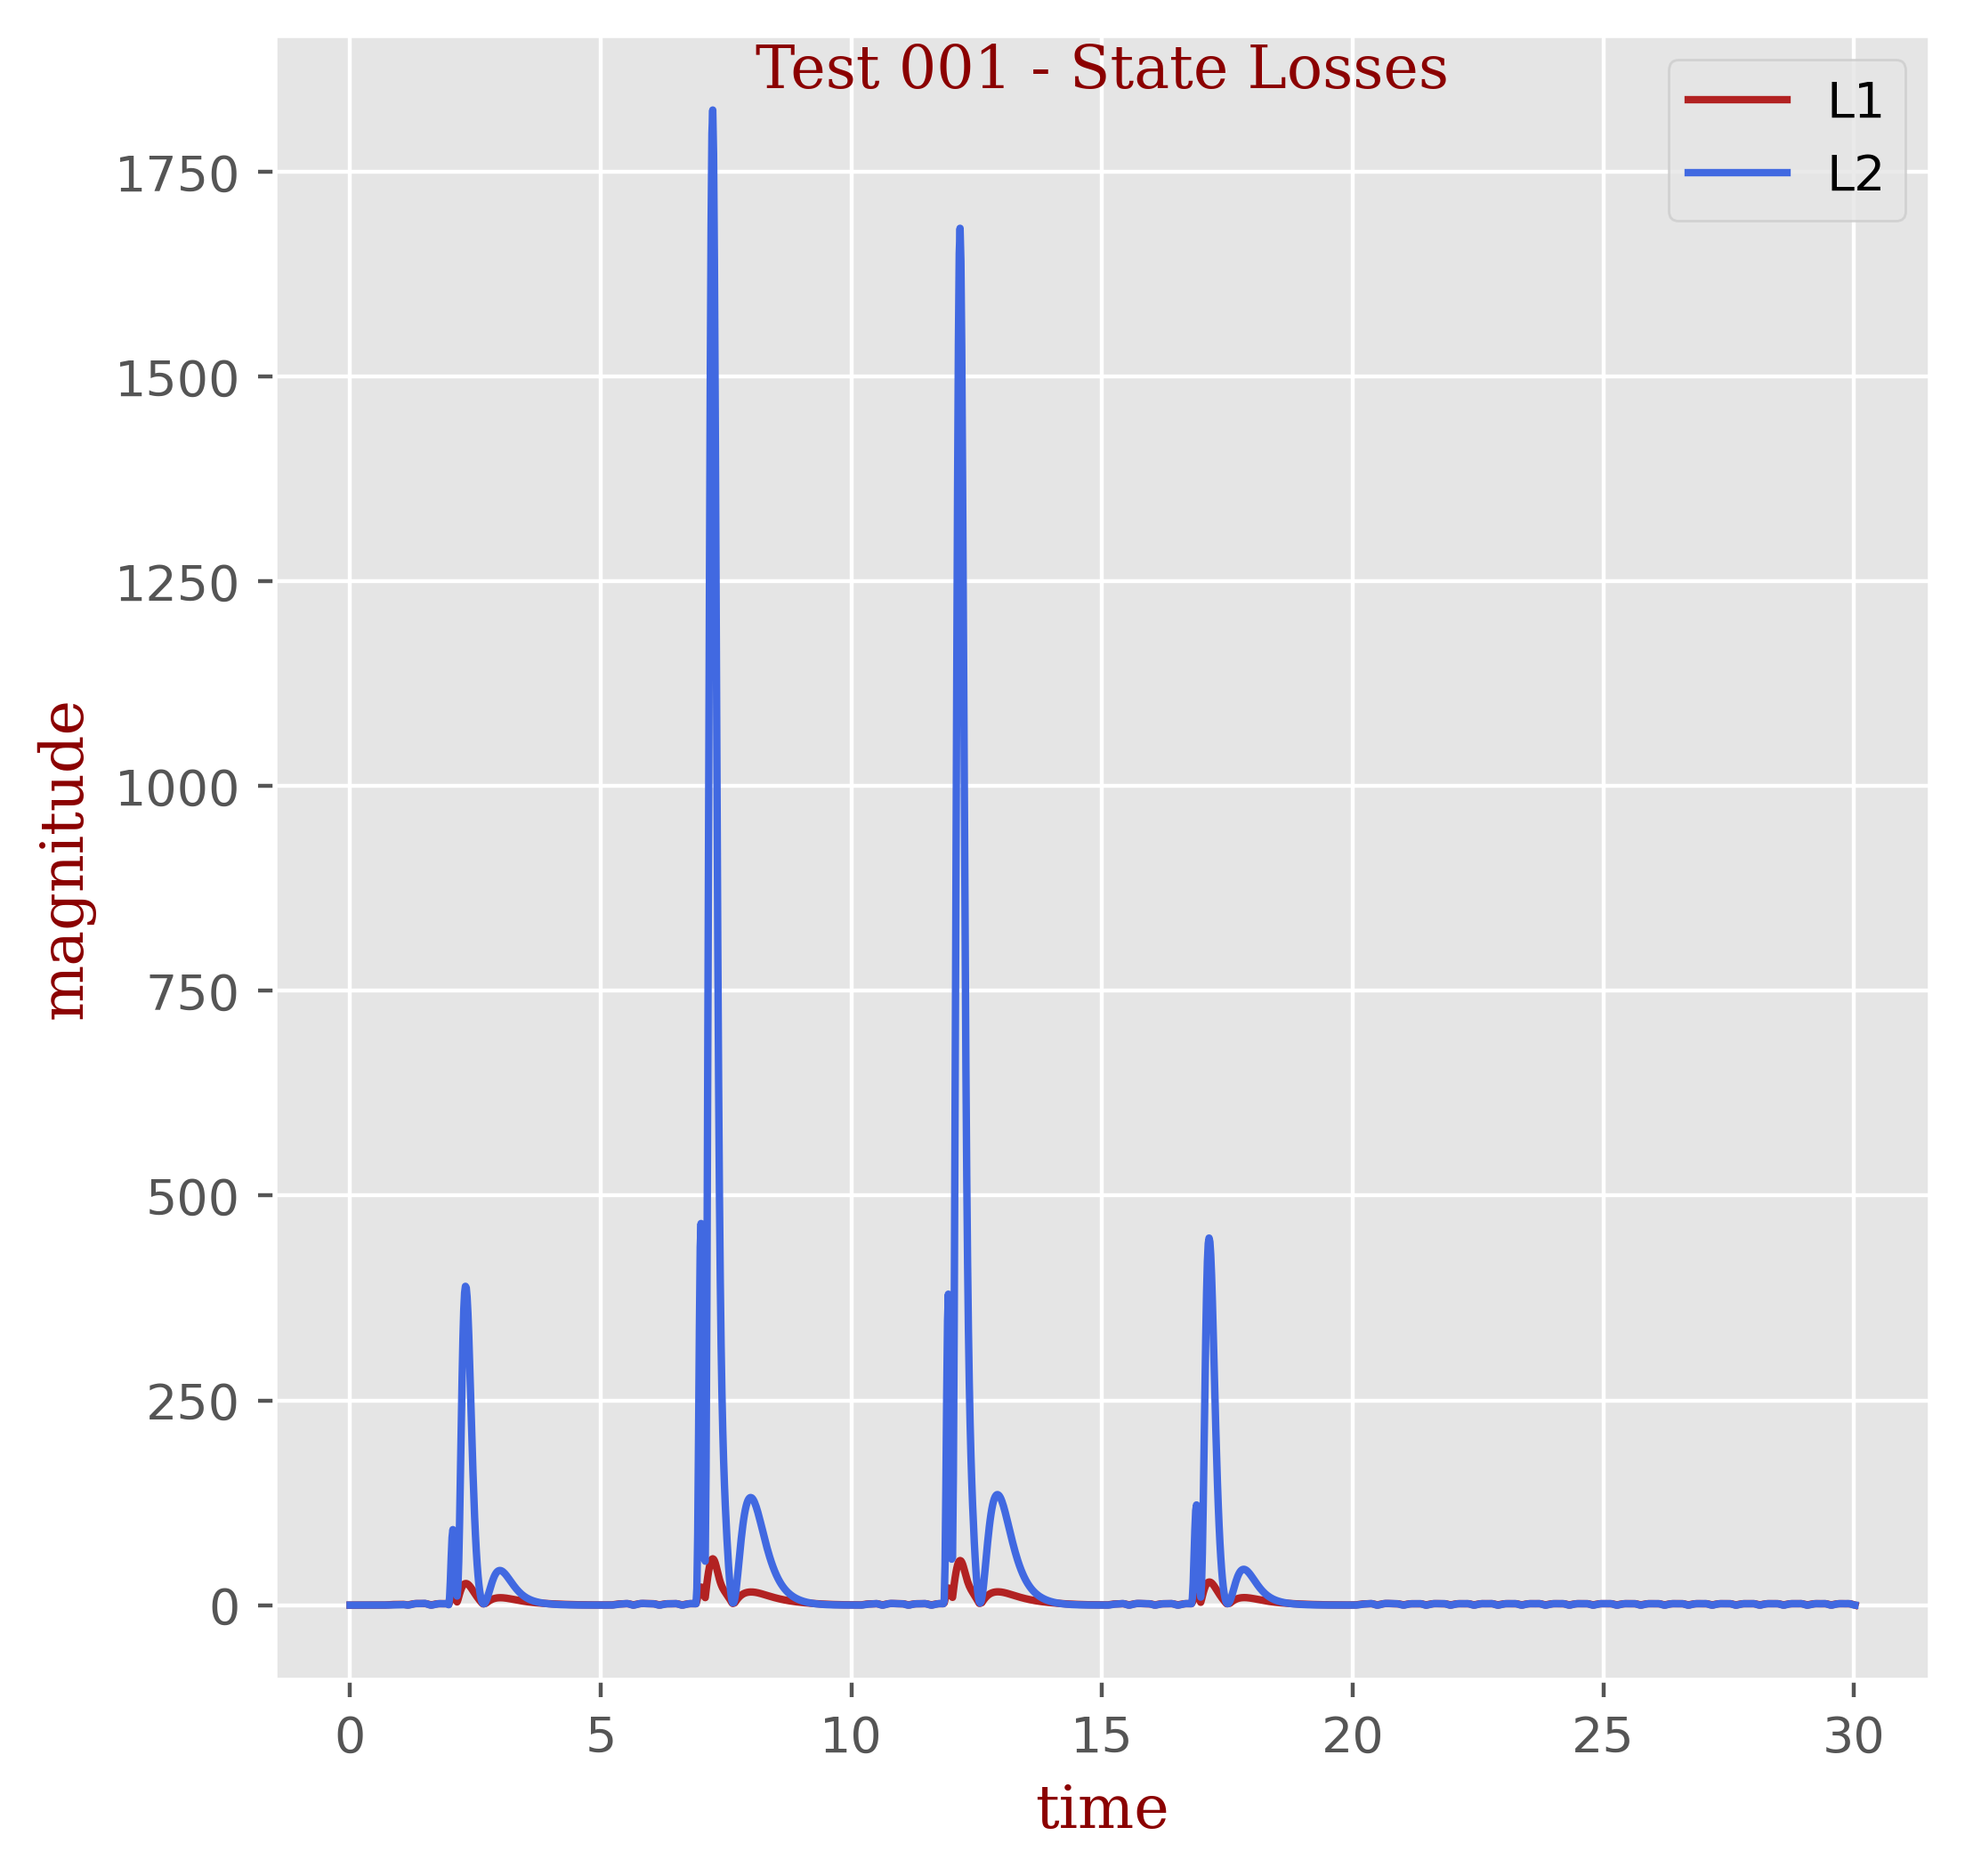
\includegraphics[width=\textwidth]{Test 001_State_Losses.png}
%         % \caption{Test 001 - Losses}
%         \label{fig_T001_los}
%     \end{subfigure}
%        \caption{Test 001}
%        \label{fig_test_001}
% \end{figure}

% \begin{figure*}[!t]
% \centerline{\subfigure[Case I]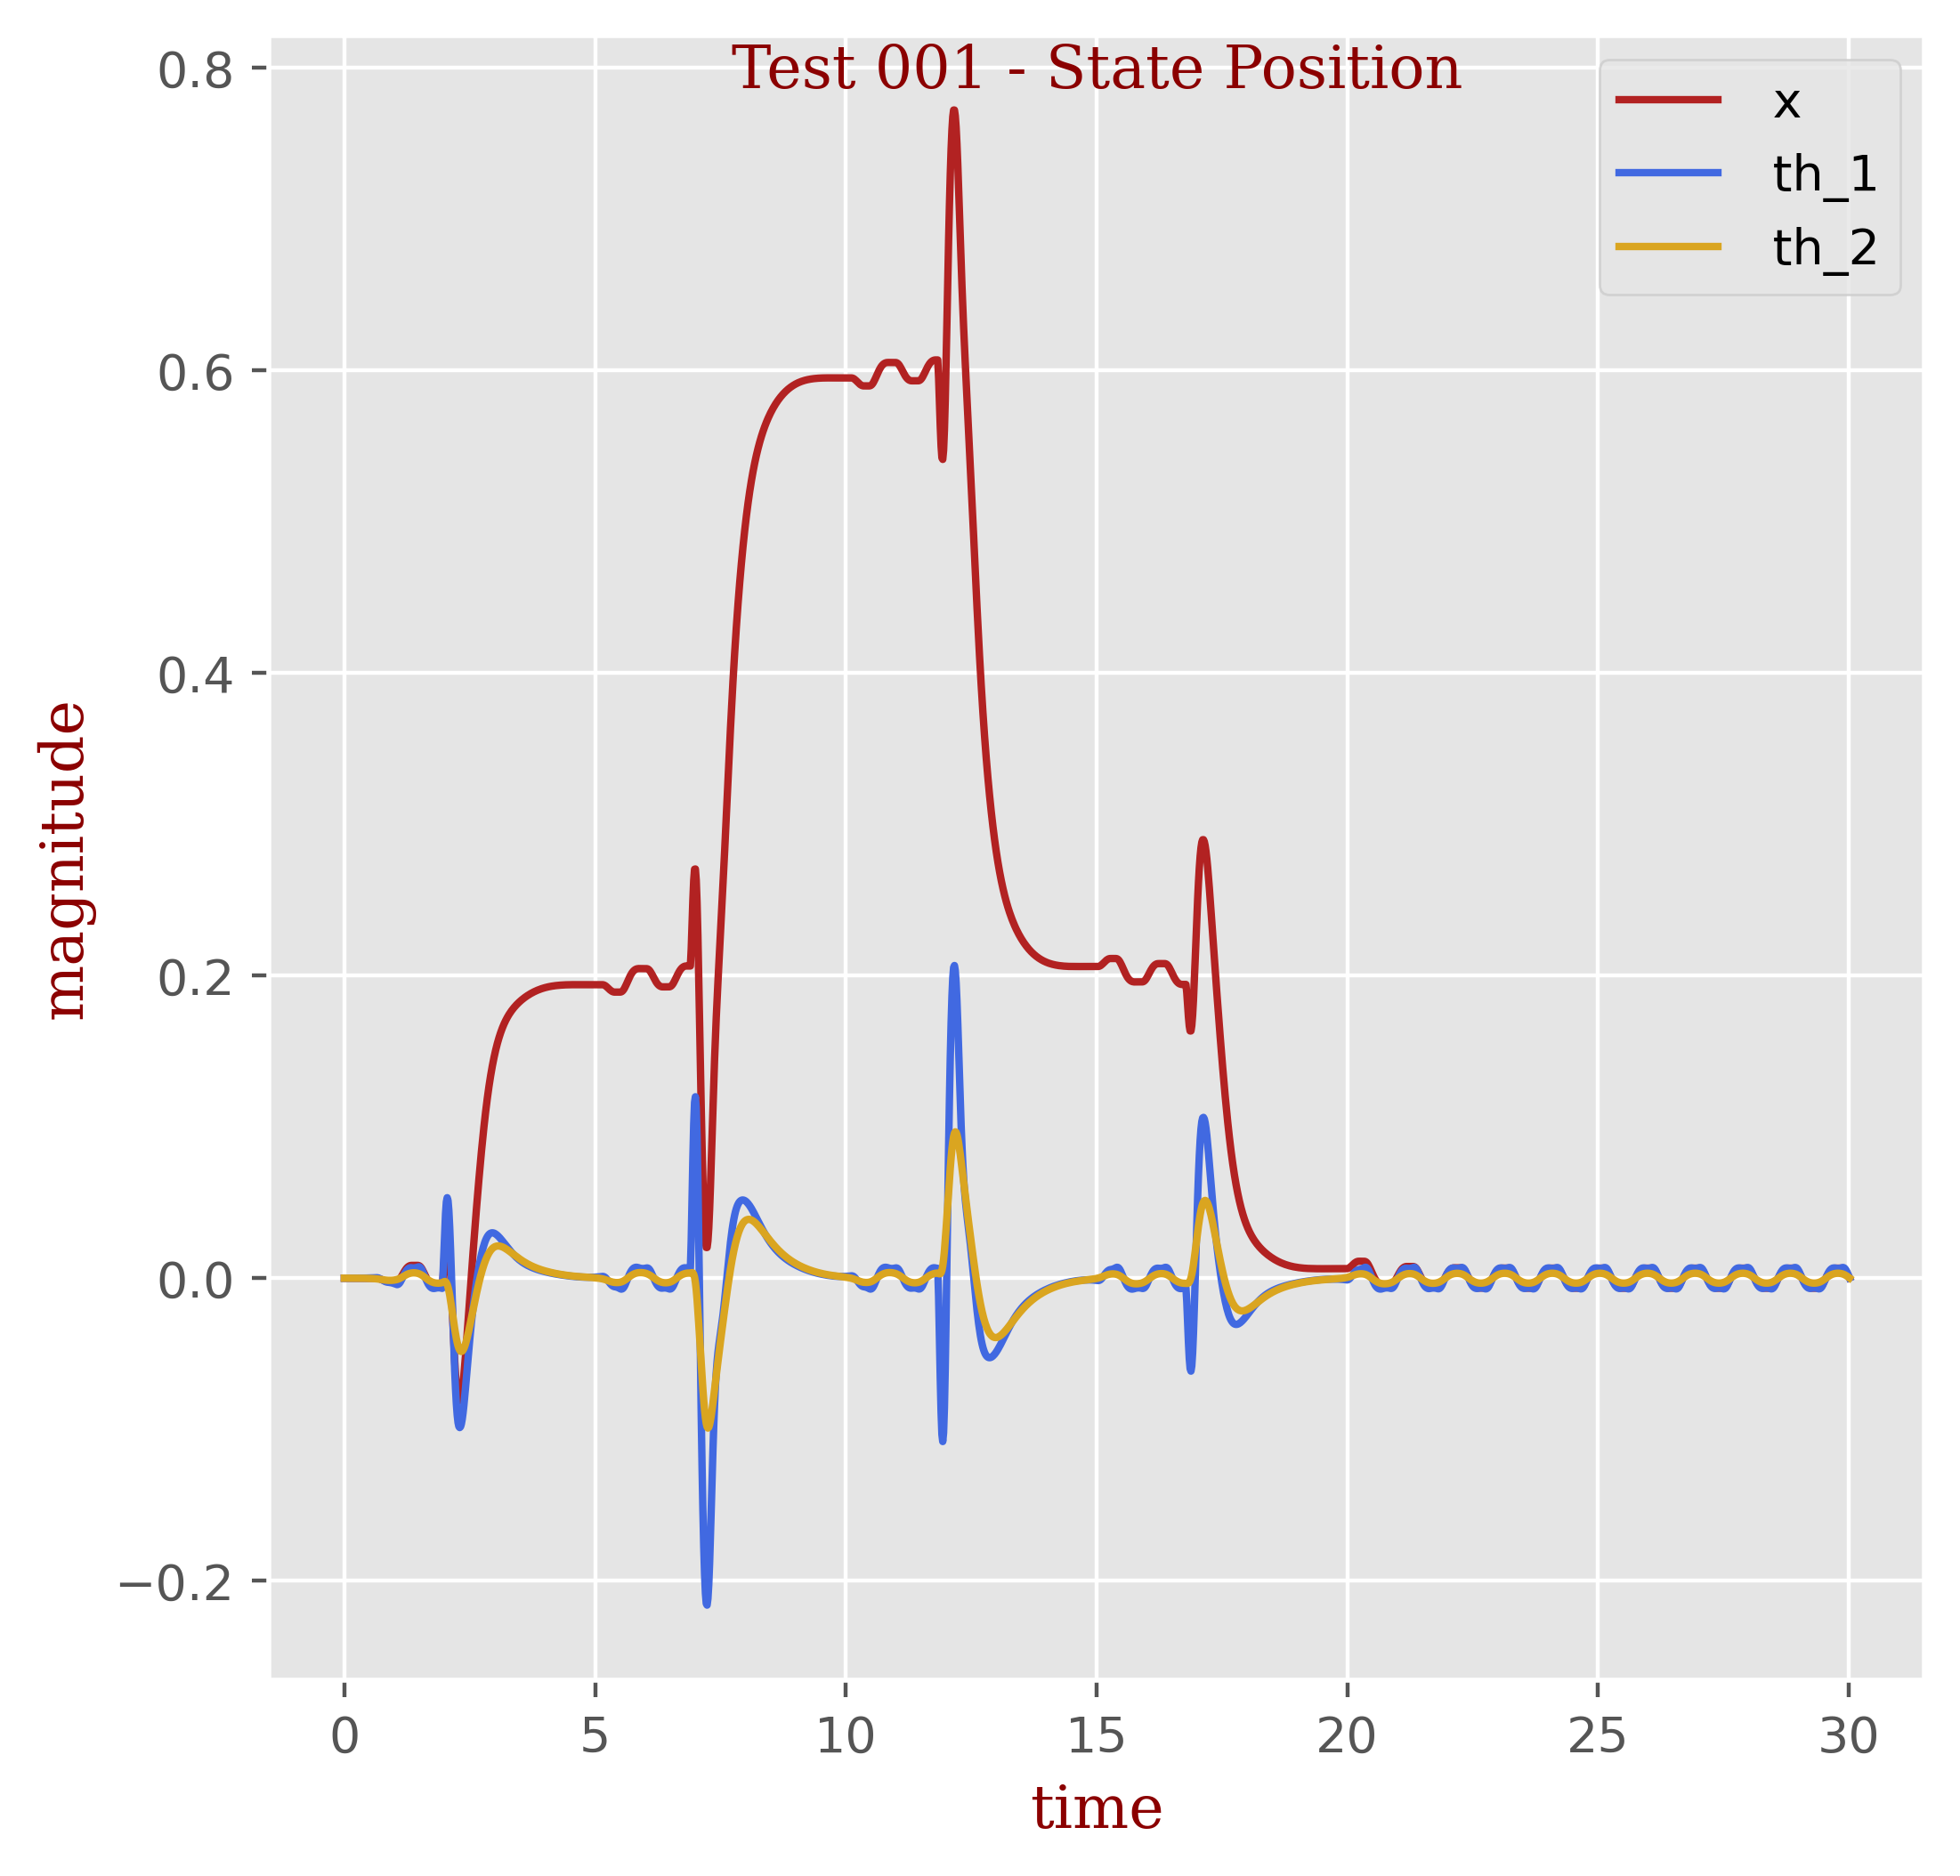
\includegraphics[width=2.5in]{Test 001_State_Position.png}%
% \label{fig_first_case}}
% \hfil
% \subfigure[Case II]{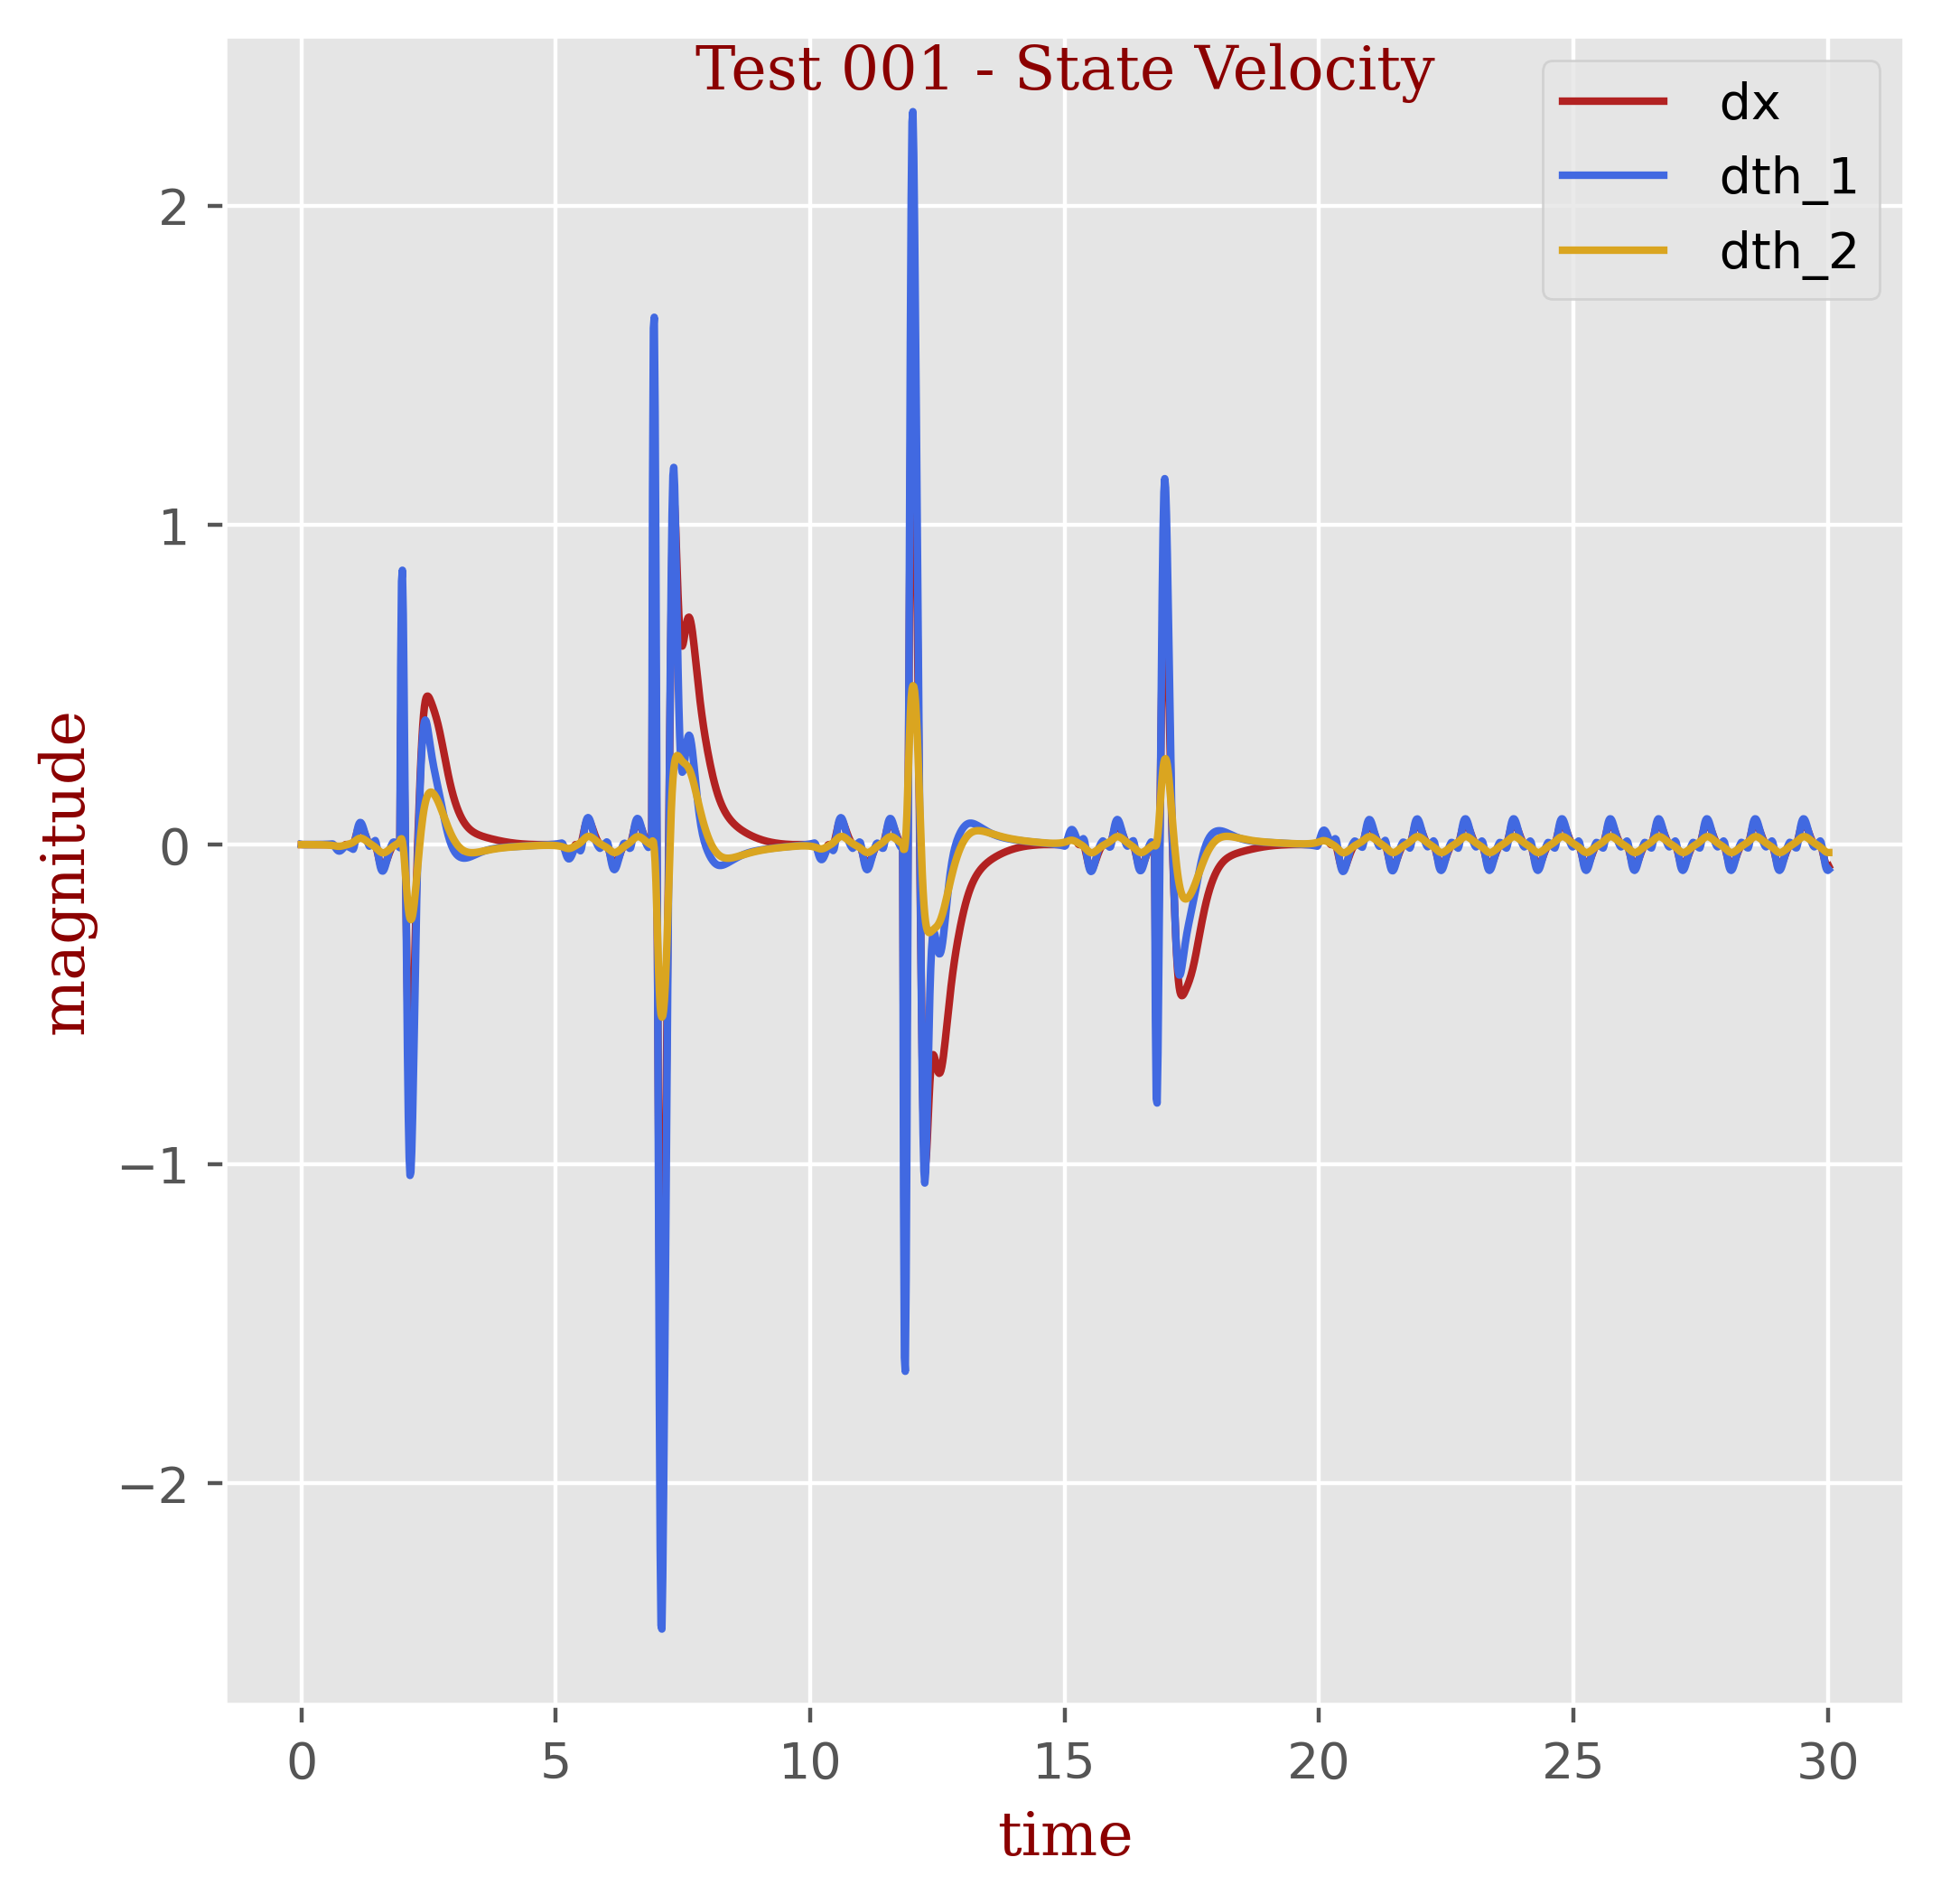
\includegraphics[width=2.5in]{Test 001_State_Velocity.png}%
% \label{fig_second_case}}
% \caption{Simulation results}
% \label{fig_sim}
% \end{figure*}
%
%
% Note that often IEEE papers with subfigures do not employ subfigure
% captions (using the optional argument to \subfloat), but instead will
% reference/describe all of them (a), (b), etc., within the main caption.



\begin{table}[!t]
\renewcommand{\arraystretch}{1.3}
\caption{Experiment I}
\label{table_001}
\centering
\begin{tabular}{|c||c|c|c|c|}
\hline
Test ID & \(l_1\) & \(m_1\) & \(l_2\) & \(m_2\) \\
\hline\hline
001 & 0.6 & 0.2 & 0.6 & 0.2 \\
002 & 0.6 & 0.3 & 0.6 & 0.2 \\
003 & 0.6 & 0.4 & 0.6 & 0.2 \\
004 & 0.6 & 0.4 & 0.6 & 0.3 \\
005 & 0.6 & 0.4 & 0.6 & 0.4 \\
006 & 0.6 & 0.3 & 0.6 & 0.4 \\
007 & 0.6 & 0.2 & 0.6 & 0.4 \\
008 & 0.6 & 0.2 & 0.5 & 0.2 \\
009 & 0.6 & 0.2 & 0.7 & 0.2 \\
010 & 0.6 & 0.2 & 0.8 & 0.2 \\
011 & 0.5 & 0.2 & 0.6 & 0.2 \\
012 & 0.4 & 0.2 & 0.6 & 0.2 \\
013 & 0.3 & 0.2 & 0.6 & 0.2 \\
014 & 0.7 & 0.2 & 0.6 & 0.2 \\
\hline
\end{tabular}
\end{table}



\begin{figure}
\centering
% \subfigure[\(q(t)\)]{\label{fig:a}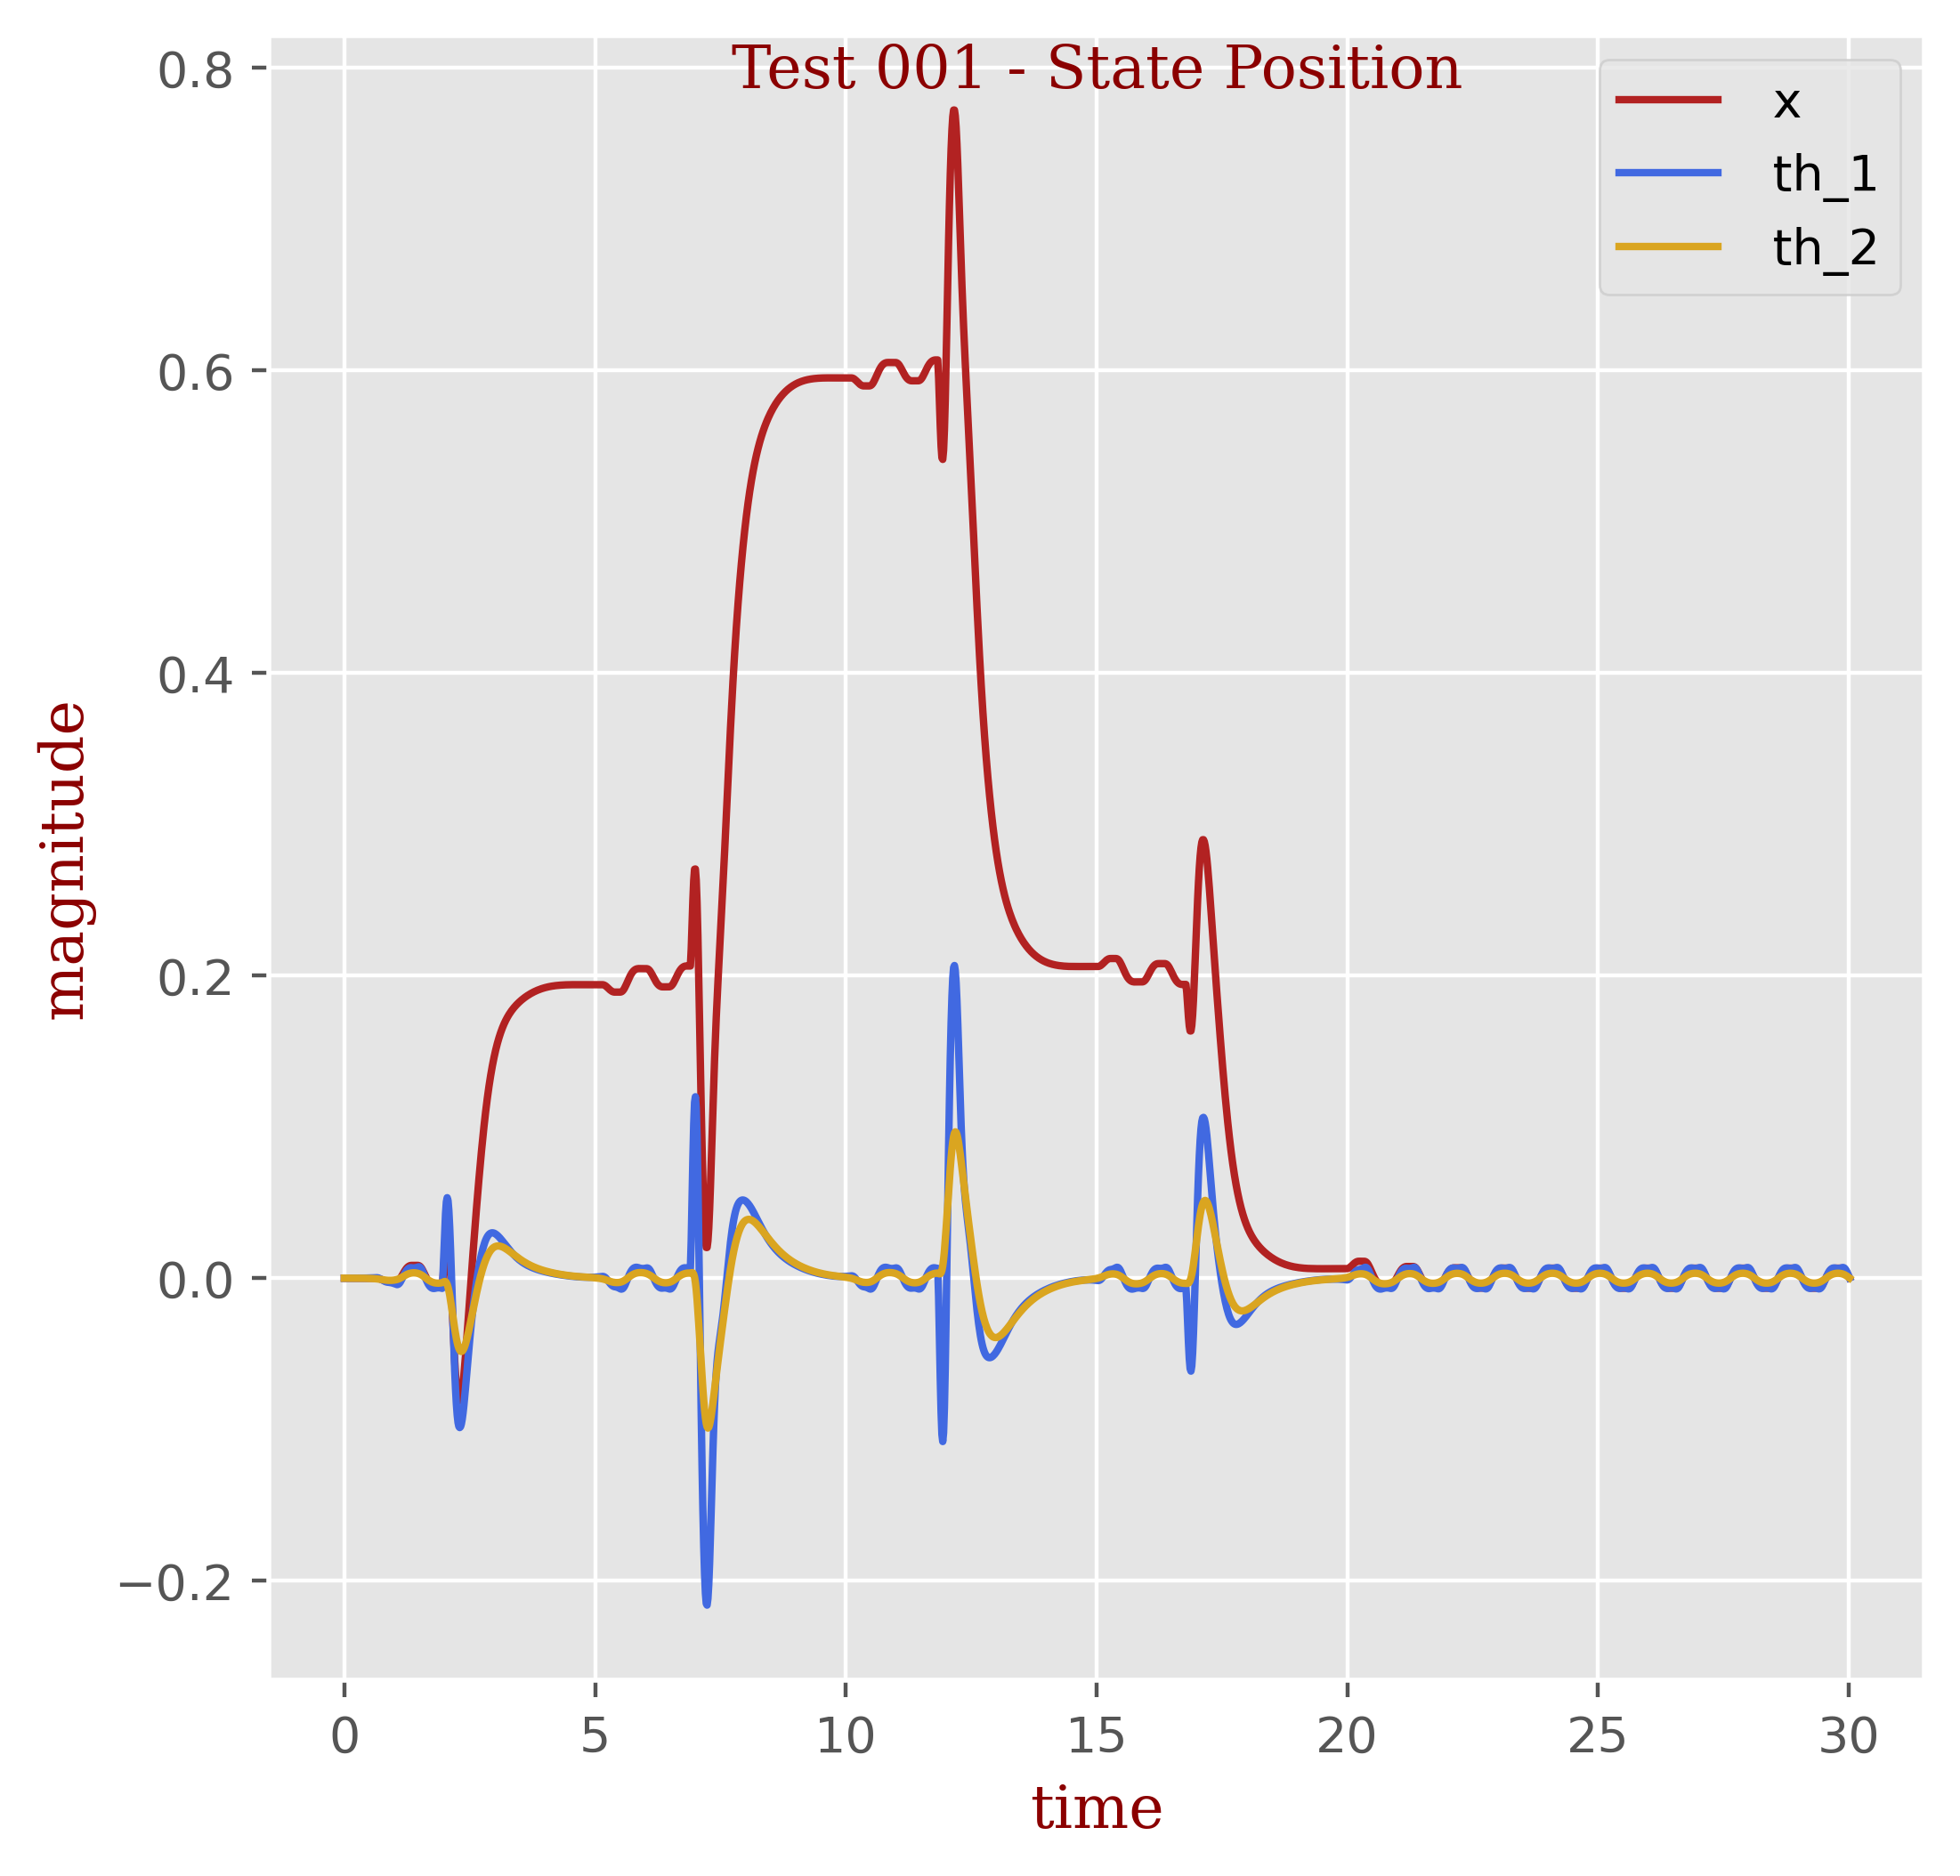
\includegraphics[width=27mm]{Test 001_State_Position.png}}
\subfigure[\(q(t)\)]{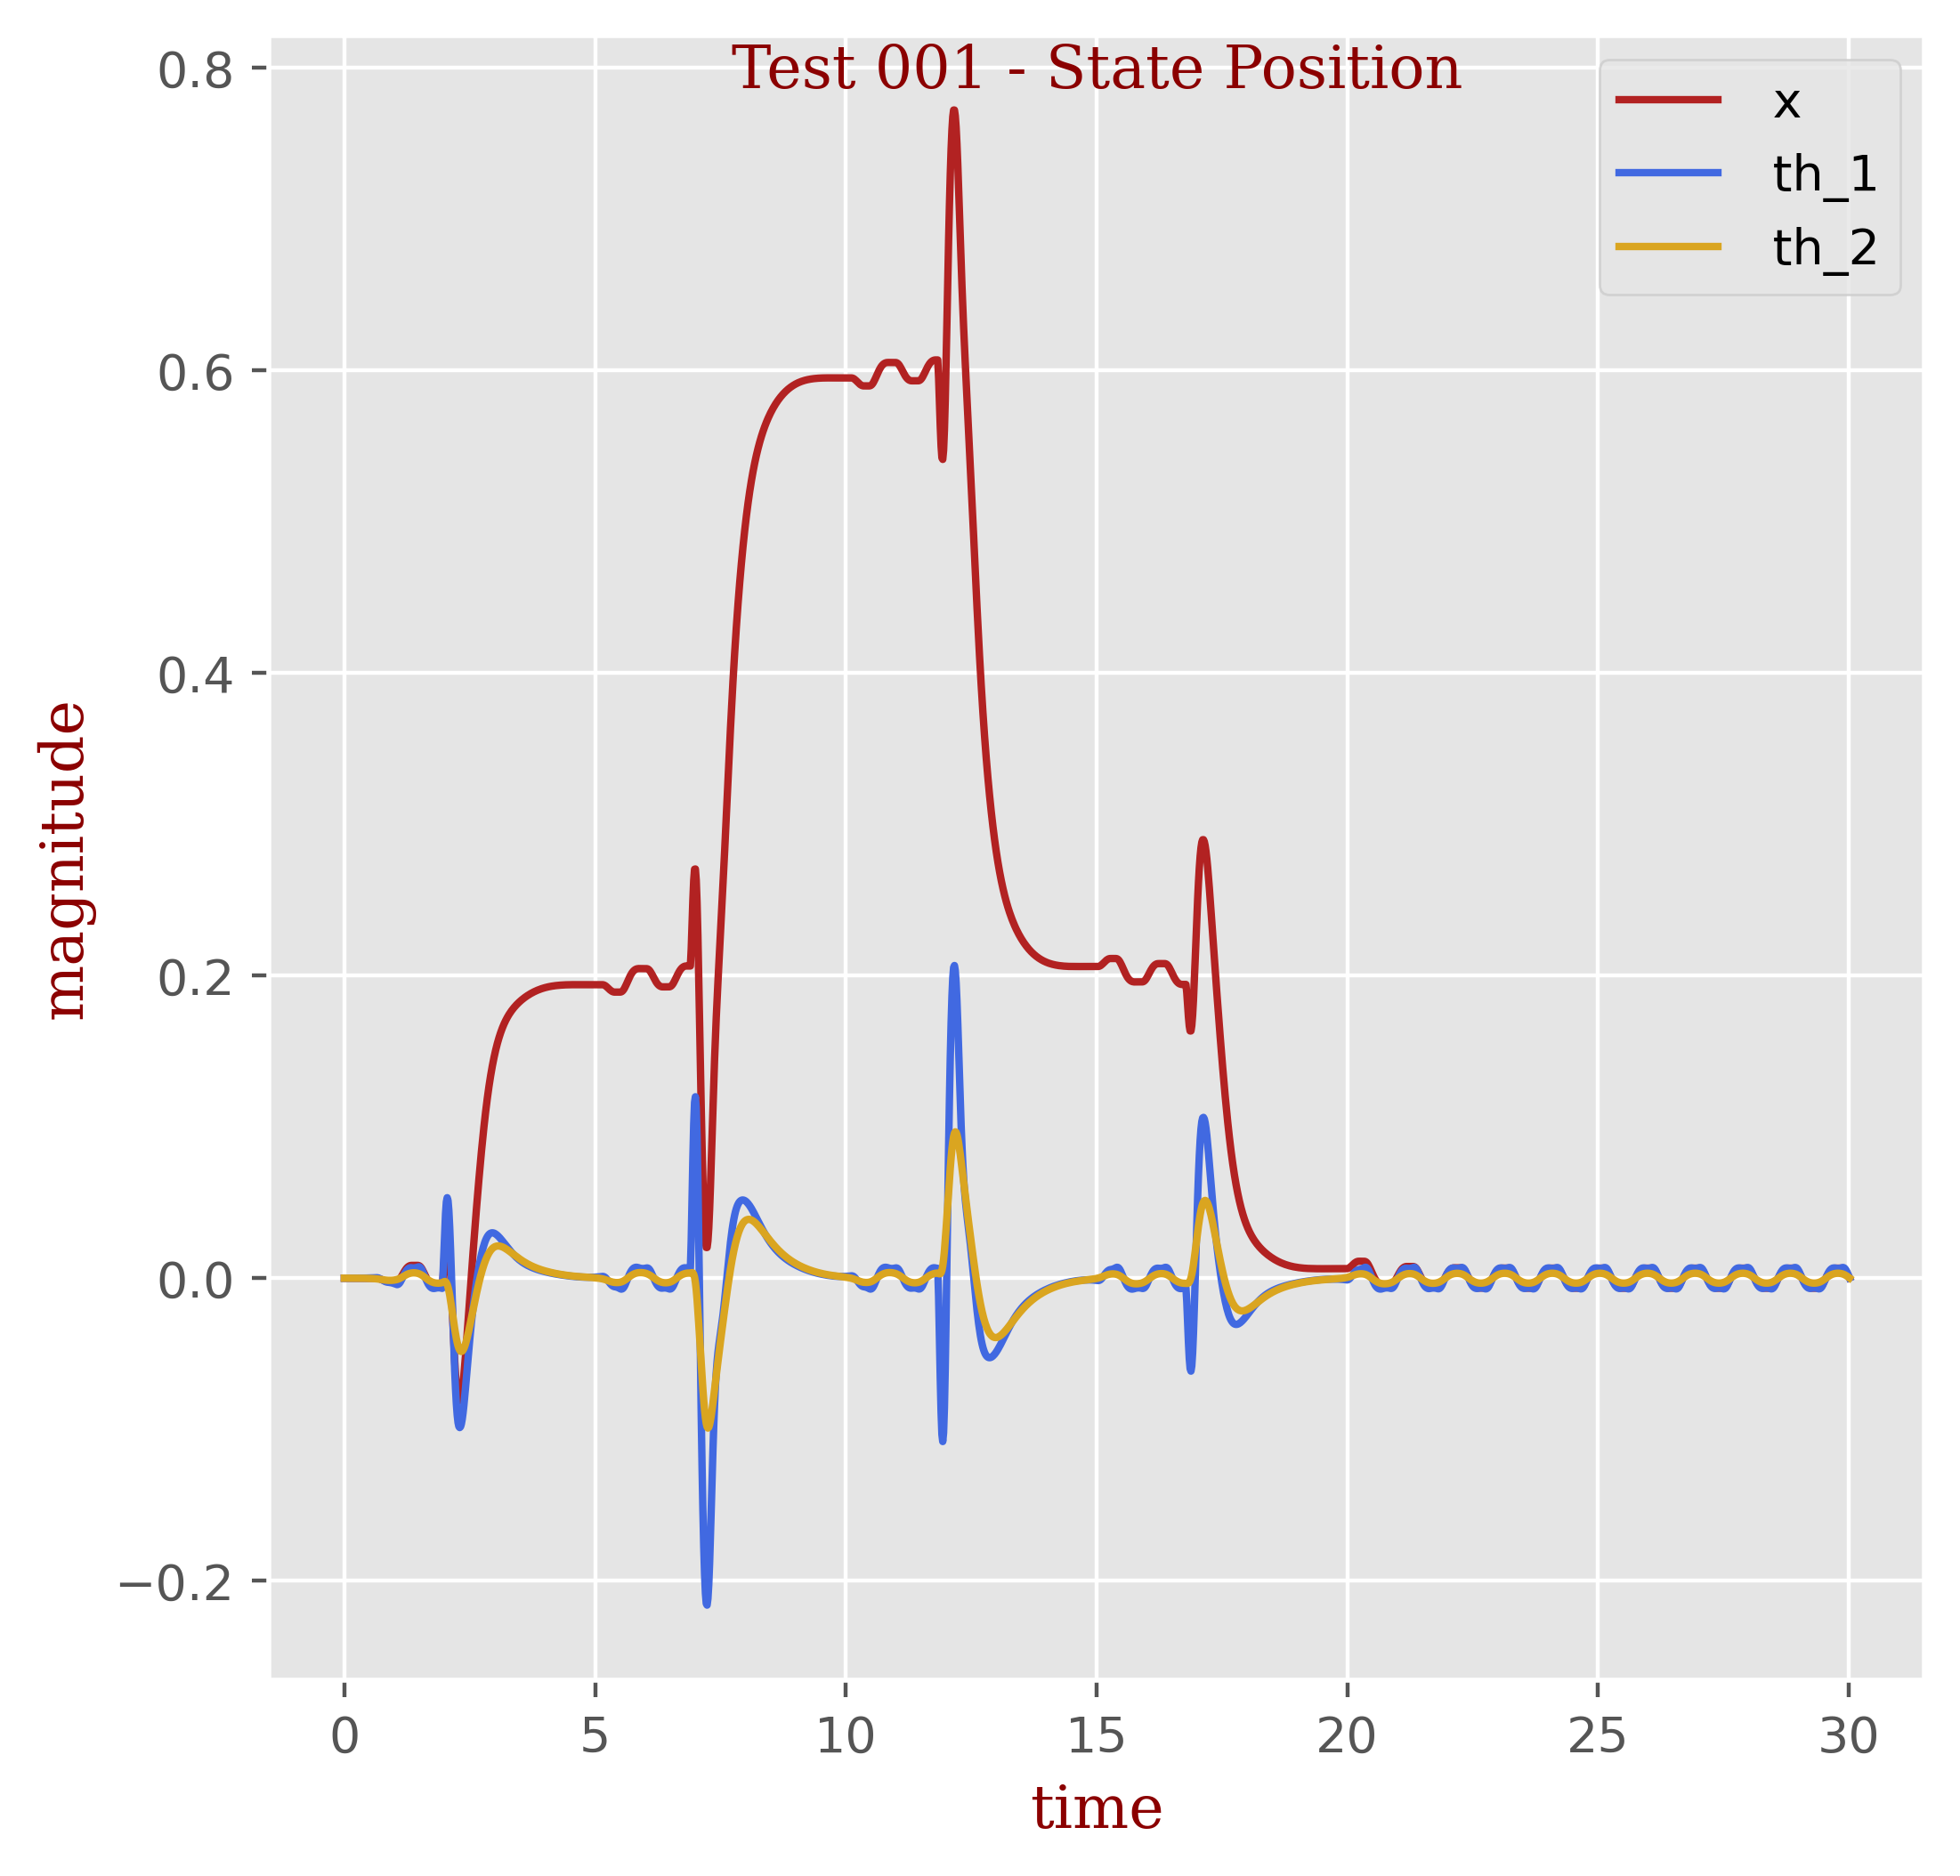
\includegraphics[width=27mm]{Test 001_State_Position.png}}
\subfigure[\(\dot{q}(t)\)]{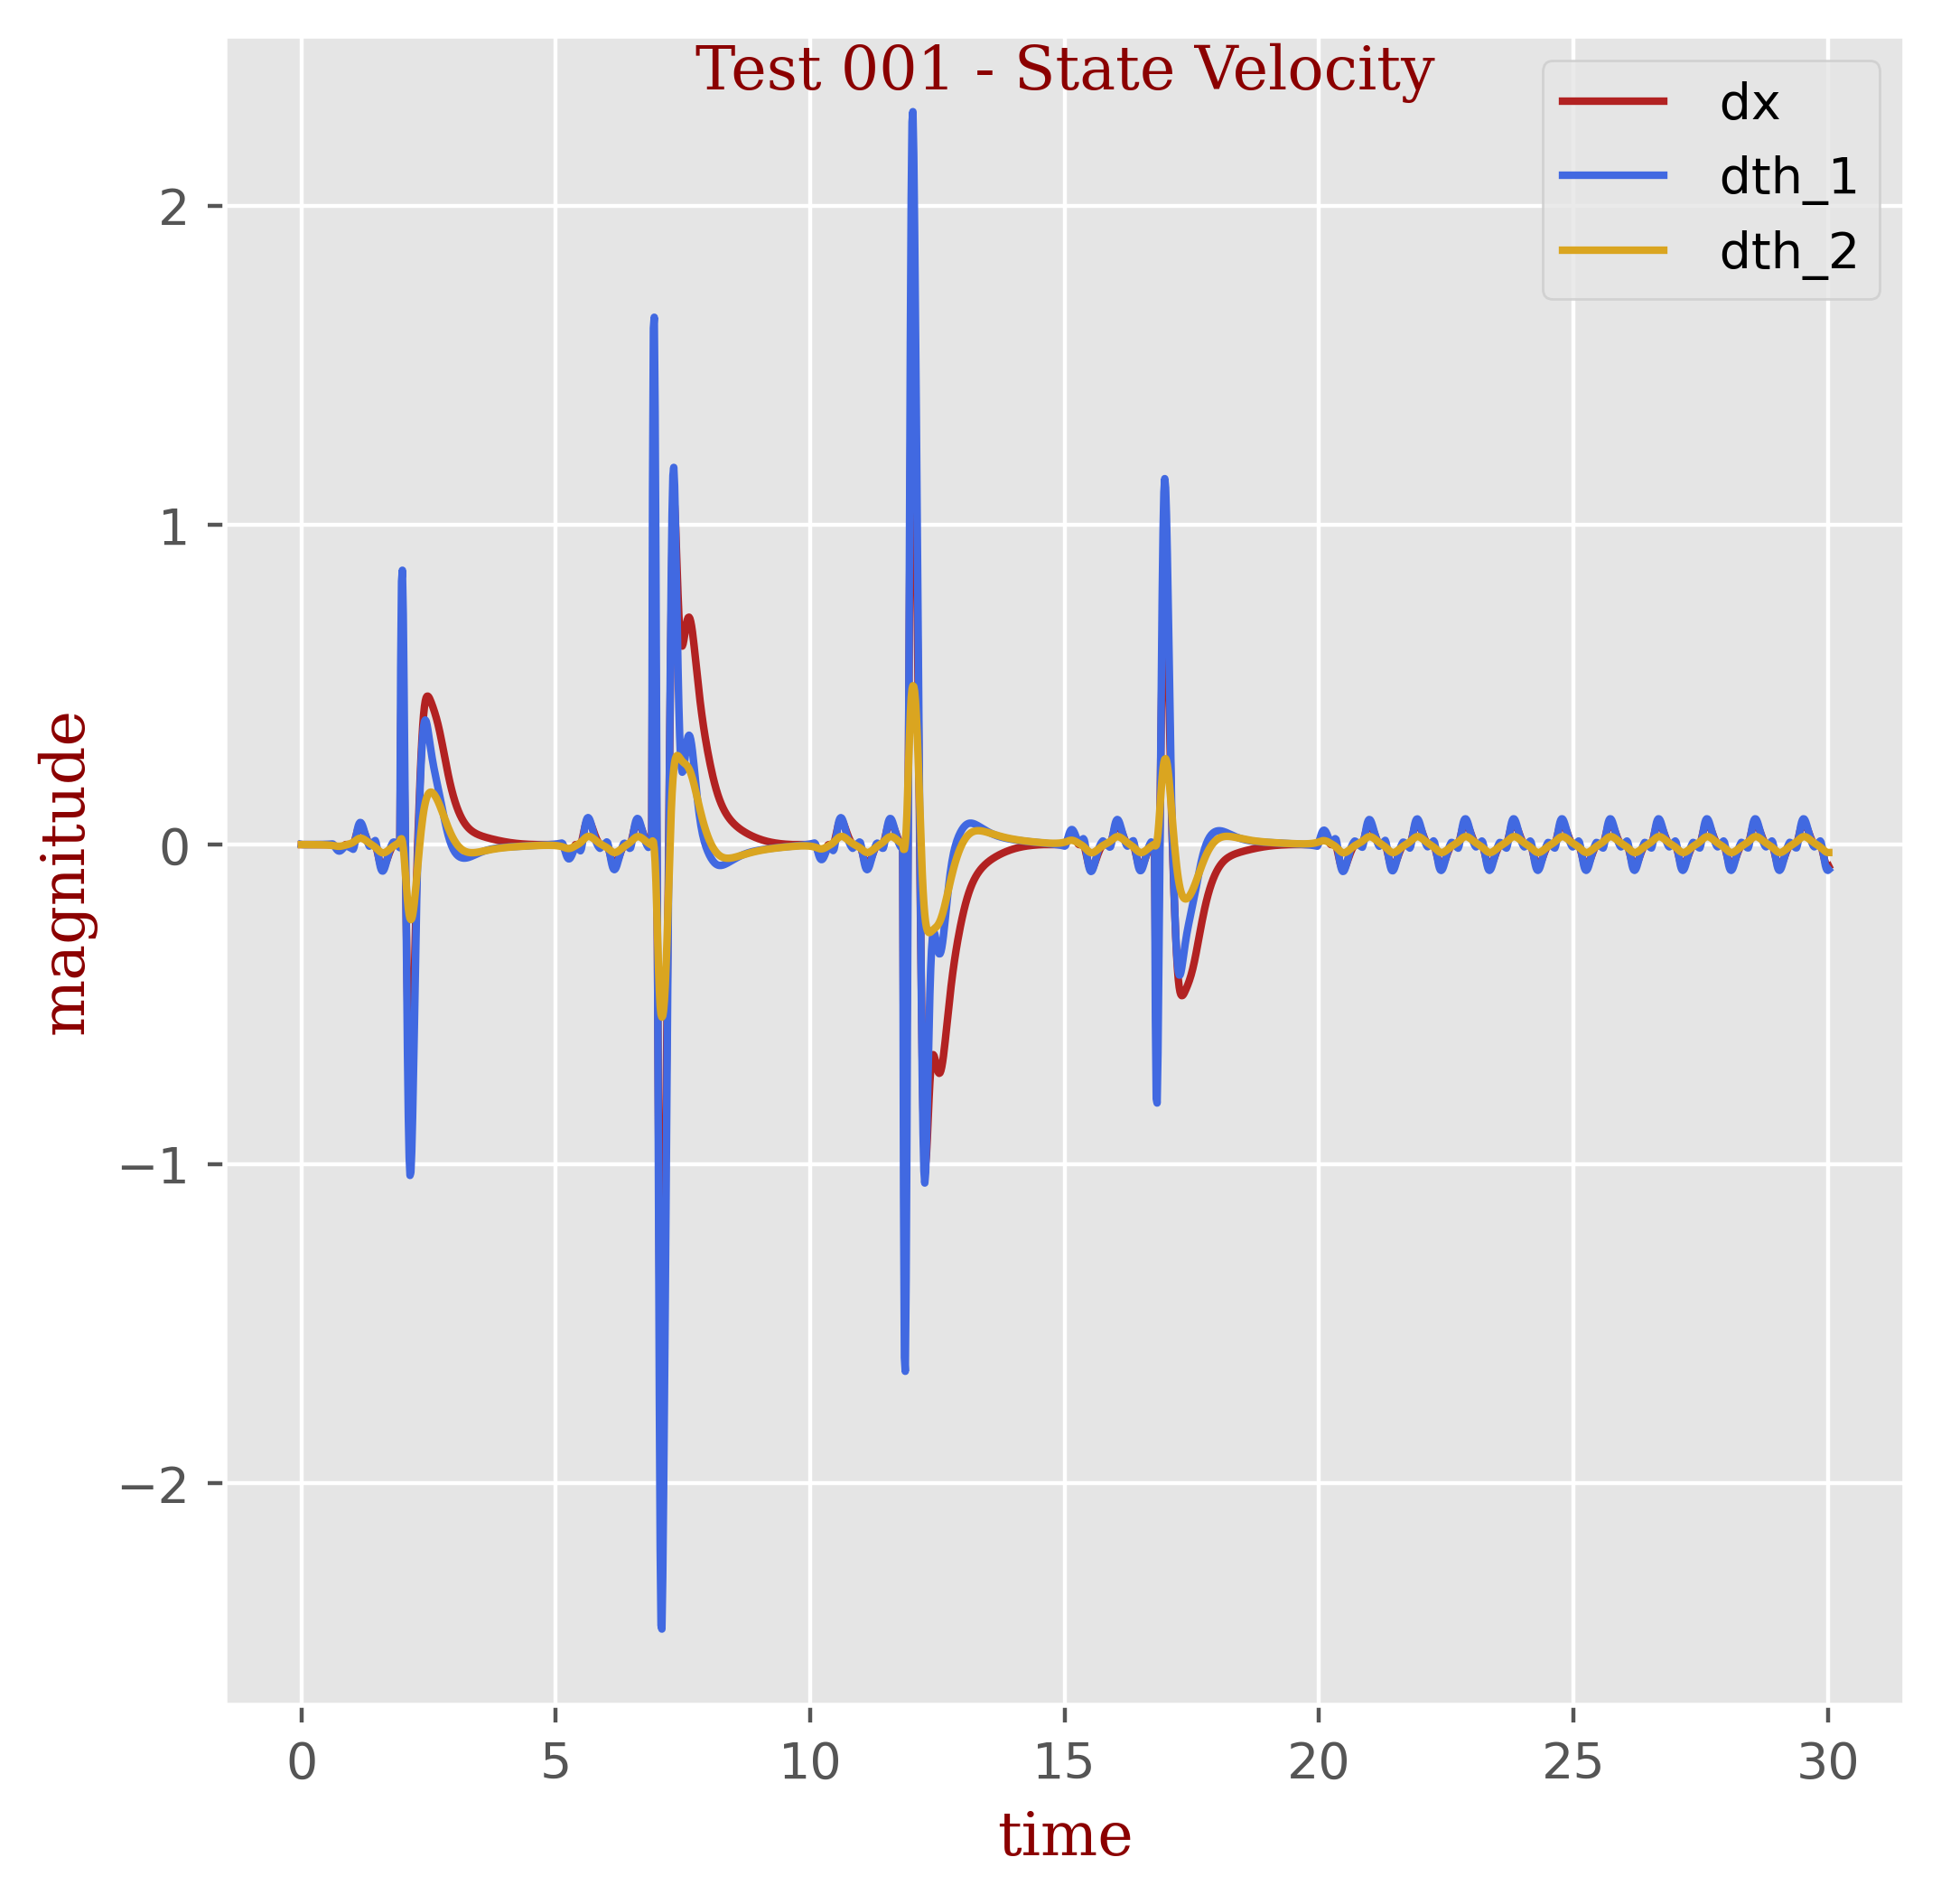
\includegraphics[width=27mm]{Test 001_State_Velocity.png}}
\subfigure[Loss]{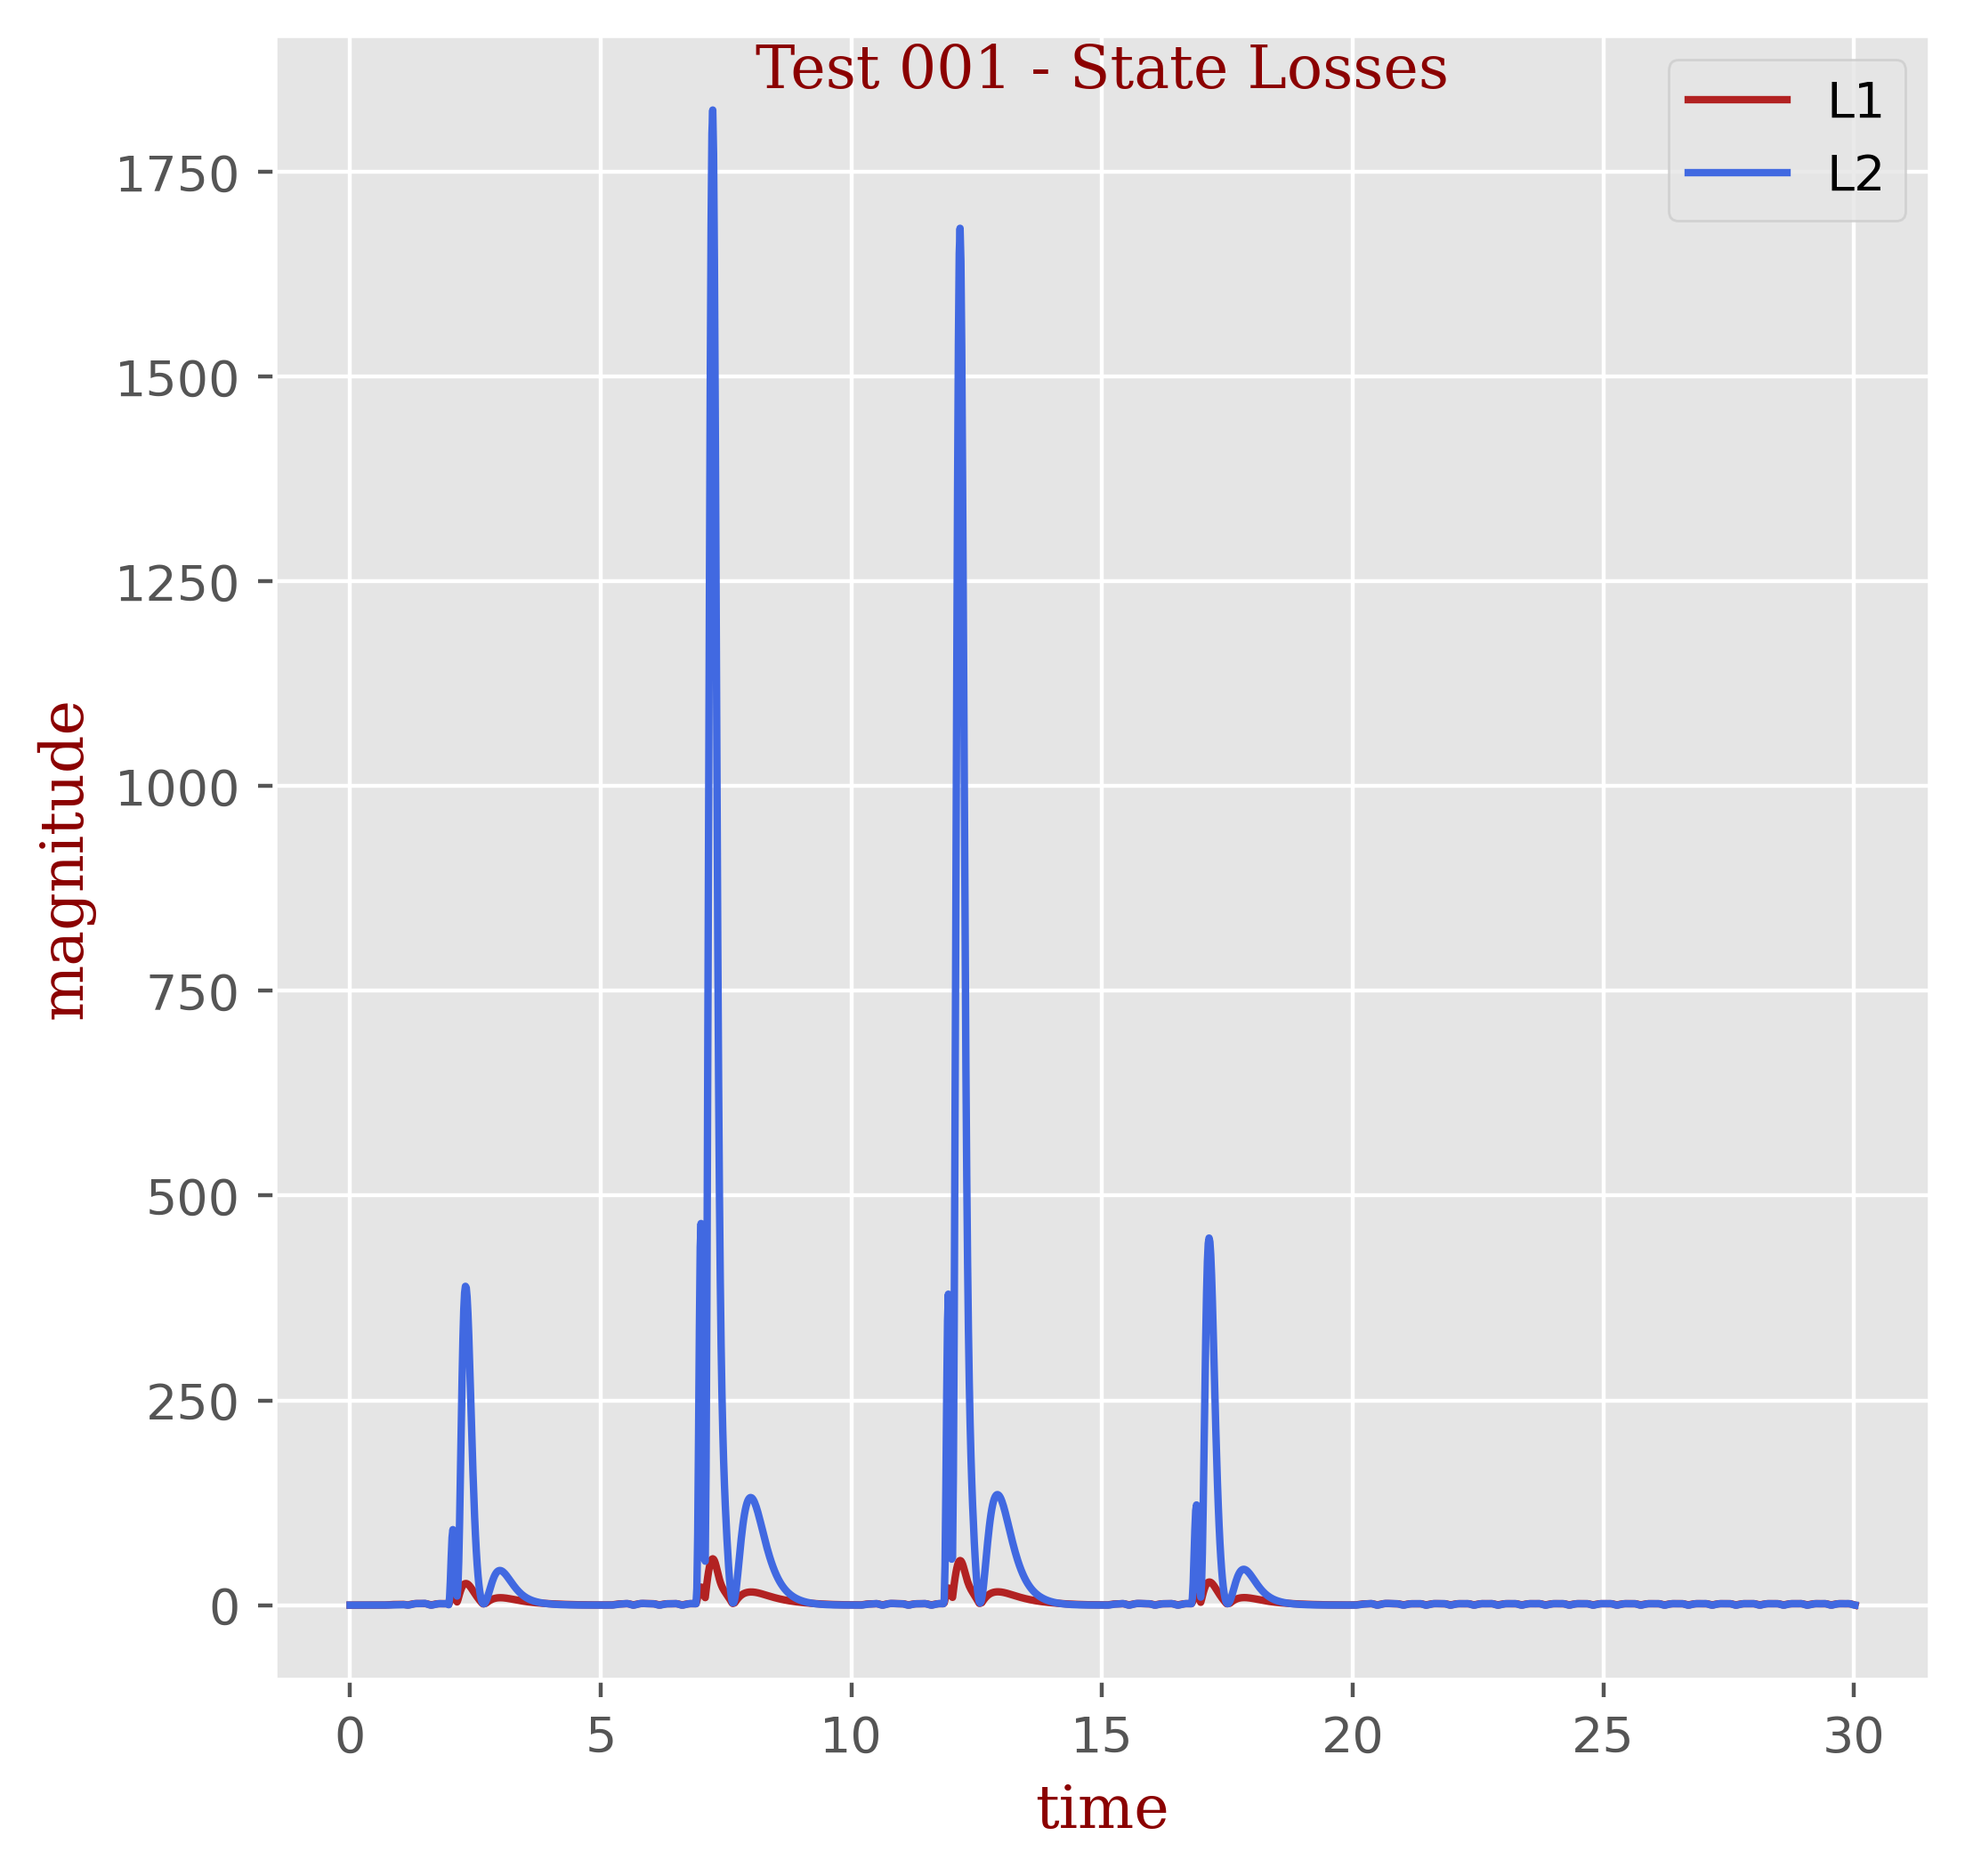
\includegraphics[width=27mm]{Test 001_State_Losses.png}}
\caption{Test 001}
\end{figure}





\section{Conclusion}
The conclusion goes here.







% \appendices
% \section{Proof of the First Zonklar Equation}
% Appendix one text goes here.

% you can choose not to have a title for an appendix
% if you want by leaving the argument blank
% \section{Appx B title}
% Appendix two text goes here.


% use section* for acknowledgement
\section*{Acknowledgment}
The authors would like to thank...


% Can use something like this to put references on a page
% by themselves when using endfloat and the captionsoff option.
% \ifCLASSOPTIONcaptionsoff
%   \newpage
% \fi

% trigger a \newpage just before the given reference
% number - used to balance the columns on the last page
% adjust value as needed - may need to be readjusted if
% the document is modified later
%\IEEEtriggeratref{8}
% The "triggered" command can be changed if desired:
%\IEEEtriggercmd{\enlargethispage{-5in}}

% references section

% can use a bibliography generated by BibTeX as a .bbl file
% BibTeX documentation can be easily obtained at:
% http://www.ctan.org/tex-archive/biblio/bibtex/contrib/doc/
% The IEEEtran BibTeX style support page is at:
% http://www.michaelshell.org/tex/ieeetran/bibtex/
%\bibliographystyle{IEEEtran}
% argument is your BibTeX string definitions and bibliography database(s)
%\bibliography{IEEEabrv,../bib/paper}
%
% <OR> manually copy in the resultant .bbl file
% set second argument of \begin to the number of references
% (used to reserve space for the reference number labels box)

%Sets the bibliography style to UNSRT and import the
% \newpage
\bibliography{ref}
\bibliographystyle{ieeetr}

% \begin{thebibliography}{1}

% \bibitem{IEEEhowto:kopka}
% H.~Kopka and P.~W. Daly, \emph{A Guide to \LaTeX}, 3rd~ed.\hskip 1em plus
%   0.5em minus 0.4em\relax Harlow, England: Addison-Wesley, 1999.

% \end{thebibliography}

% biography section
%
% If you have an EPS/PDF photo (graphicx package needed) extra braces are
% needed around the contents of the optional argument to biography to prevent
% the LaTeX parser from getting confused when it sees the complicated
% \includegraphics command within an optional argument. (You could create
% your own custom macro containing the \includegraphics command to make things
% simpler here.)
%\begin{biography}[{\includegraphics[width=1in,height=1.25in,clip,keepaspectratio]{mshell}}]{Michael Shell}
% or if you just want to reserve a space for a photo:

% \begin{IEEEbiography}{Michael Shell}
% Biography text here.
% \end{IEEEbiography}

% % if you will not have a photo at all:
% \begin{IEEEbiographynophoto}{John Doe}
% Biography text here.
% \end{IEEEbiographynophoto}

% insert where needed to balance the two columns on the last page with
% biographies
%\newpage


% You can push biographies down or up by placing
% a \vfill before or after them. The appropriate
% use of \vfill depends on what kind of text is
% on the last page and whether or not the columns
% are being equalized.

%\vfill

% Can be used to pull up biographies so that the bottom of the last one
% is flush with the other column.
%\enlargethispage{-5in}



% that's all folks
\end{document}
